%# -*- coding: utf-8-unix -*-
%%==================================================
%% thesis.tex
%%==================================================

% 双面打印

\documentclass[doctor, fontset=adobe, openright, twoside]{sjtuthesis}
% \documentclass[bachelor, fontset=adobe, openany, oneside, submit]{sjtuthesis} 
% \documentclass[master, adobefonts, review]{sjtuthesis} 
% \documentclass[%
%   bachelor|master|doctor,	% 必选项
%   fontset=adobe|windows,  	% 只测试了adobe
%   oneside|twoside,		% 单面打印,双面打印(奇偶页交换页边距,默认)
%   openany|openright, 		% 可以在奇数或者偶数页开新章|只在奇数页开新章(默认)
%   zihao=-4|5,, 		% 正文字号:小四、五号(默认)
%   review,	 		% 盲审论文,隐去作者姓名、学号、导师姓名、致谢、发表论文和参与的项目
%   submit			% 定稿提交的论文,插入签名扫描版的原创性声明、授权声明 
% ]

% 逐个导入参考文献数据库
\addbibresource{bib/thesis.bib}
% \addbibresource{bib/chap2.bib}
\usepackage{booktabs}
\begin{document}

%% 无编号内容:中英文论文封面、授权页
%# -*- coding: utf-8-unix -*-
\title{上海交通大学学位论文}
\author{肖\quad{}敏}
\advisor{邬晶副教授}
% \coadvisor{某某教授}
\defenddate{2017年2月15日}
\school{上海交通大学}
\institute{自动化系}
\studentnumber{1140329109}
\major{控制工程专业}

\englishtitle{过程控制系统的入侵检测和防御}
\englishauthor{\textsc{Min Xiao}}
\englishadvisor{A.P. \textsc{Jing Wu}}
% \englishcoadvisor{Prof. \textsc{Uom Uom}}
\englishschool{Shanghai Jiao Tong University}
\englishinstitute{\textsc{Depart of Automation, School of Electronic, Information and Electrical Engineering} \\
  \textsc{Shanghai Jiao Tong University} \\
  \textsc{Shanghai, P.R.China}}
\englishmajor{Control Engineering}
\englishdate{Feb. 15th, 2017}


\maketitle

\makeenglishtitle

\makeatletter
\ifsjtu@submit\relax
	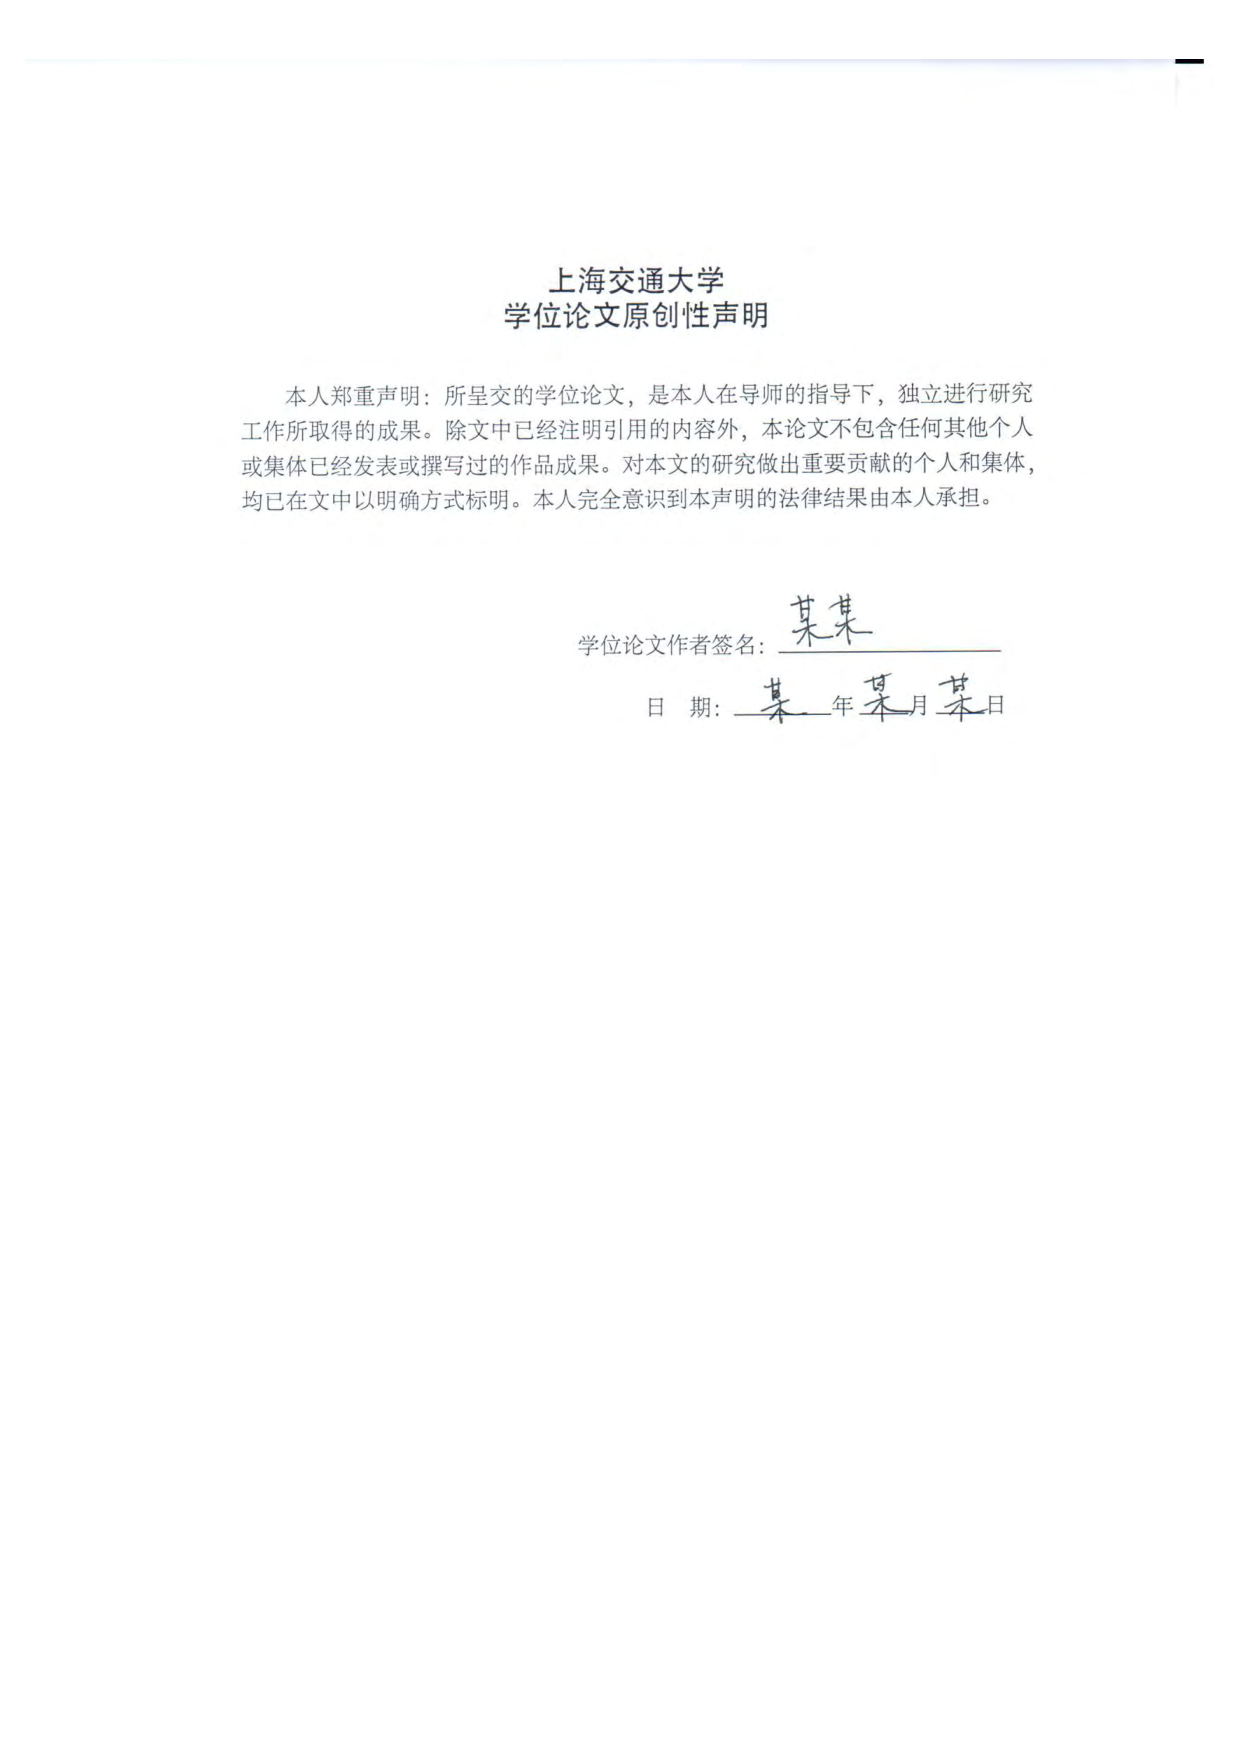
\includepdf{pdf/original.pdf}
	\cleardoublepage
	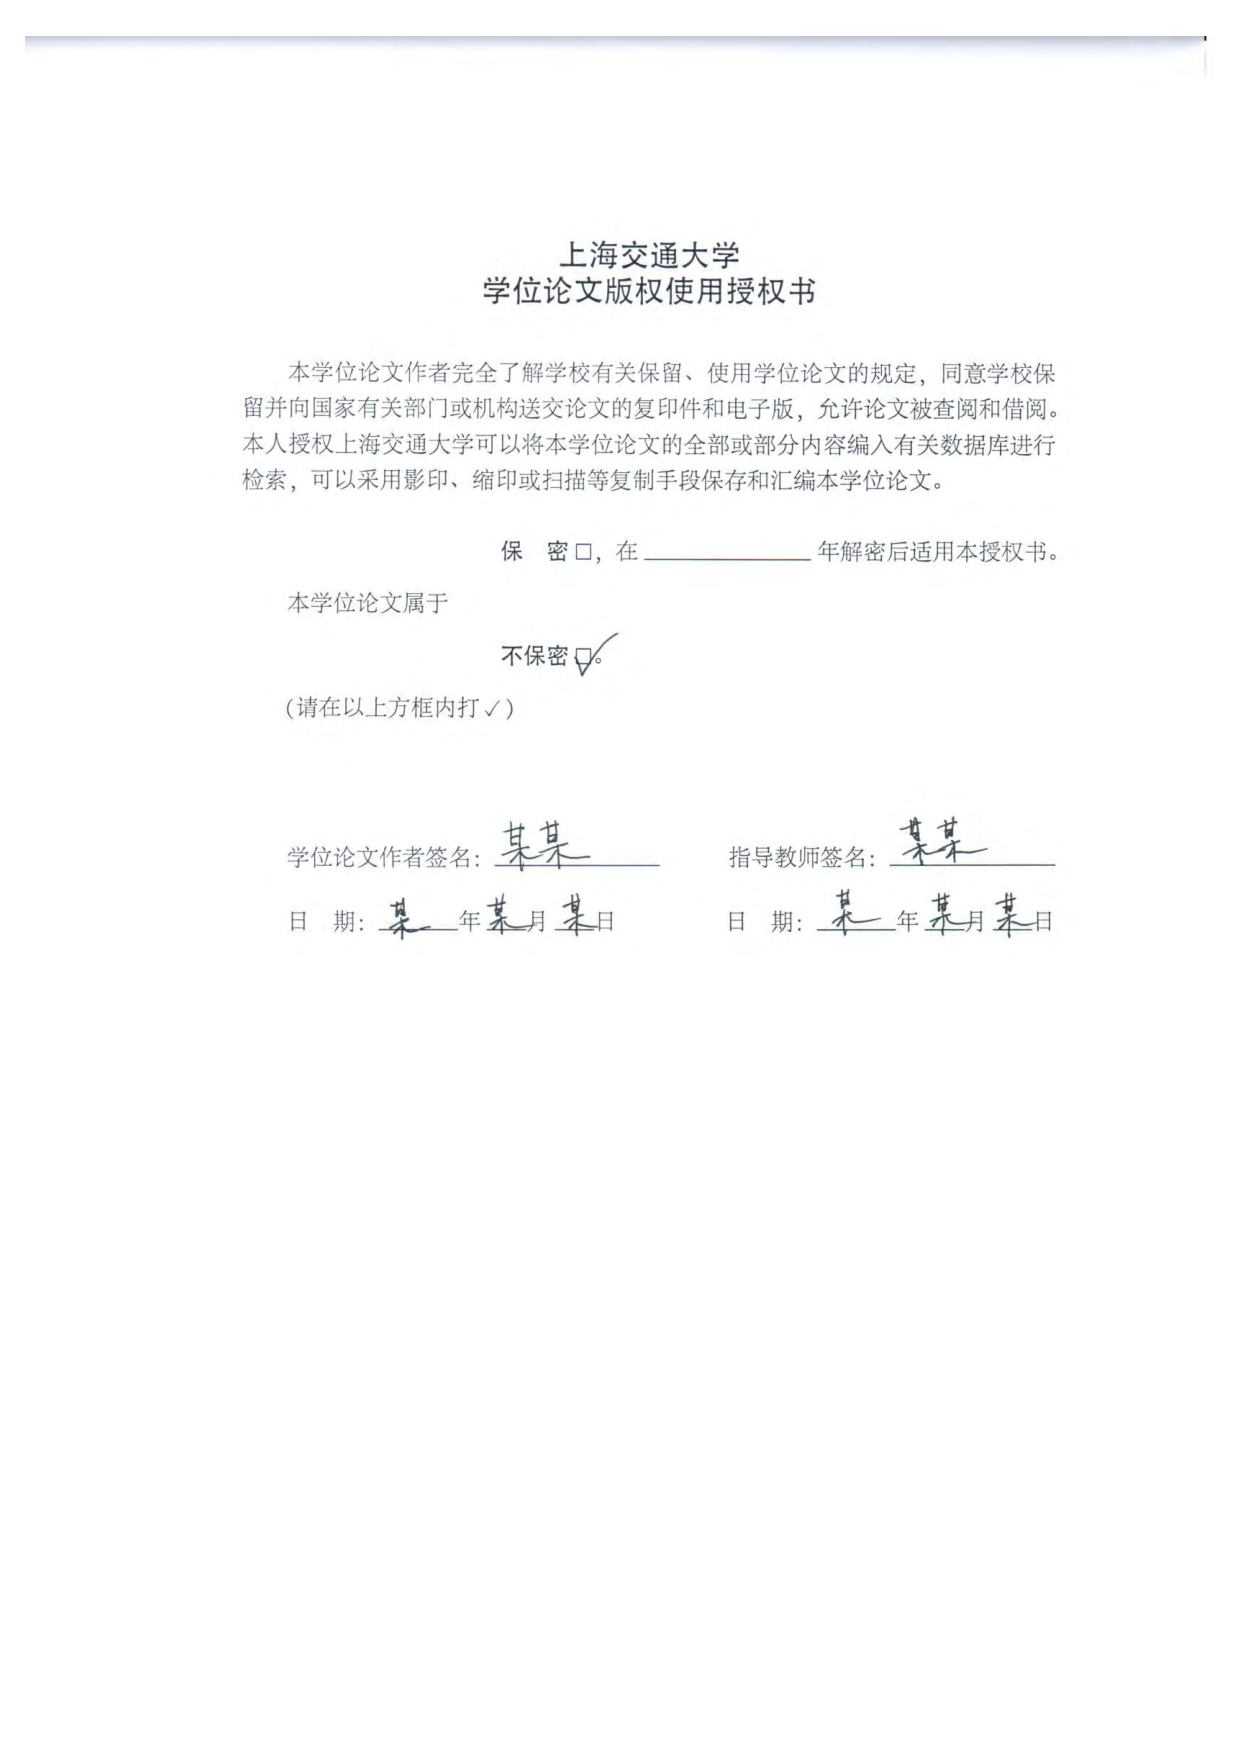
\includepdf{pdf/authorization.pdf}
	\cleardoublepage
\else
	\makeDeclareOriginal
	\makeDeclareAuthorization
\fi
\makeatother


\frontmatter 	% 使用罗马数字对前言编号

%% 摘要
\pagestyle{main}
%# -*- coding: utf-8-unix -*-
%%==================================================
%% abstract.tex for SJTU Master Thesis
%%==================================================

\begin{abstract}
过程控制系统(PCS, Process Control Systems)的网络物理安全问题正在变得日趋严重,不管是从网络信息安全还是从物理数据完整性的角度,PCS所面临的安全风险和入侵威胁都在不断增加,而且伴随着工业安全事故的数量逐年增加,相应带来的破坏和灾难也越发严重。所以,PCS的网络信息安全和数据安全已经成为越来越需要全面和深入研究的国家基础设施和关键领域。正是在这种背景下,为了检测对PCS系统的入侵威胁,建立安全系统和关键国家基础设施安全的综合防御系统,本文针对PCS网络物理安全的入侵类型、控制器本身及其与物理设备交互数据的脆弱性特点,在面向PCS的攻击和入侵检测方法的研究和设计方面主要做了以下工作:
\begin{enumerate}
	\item 构造了基于故障检测机制错误序列注入(FSI)攻击,其可以避开现有的系统故障检测机制,通过感染和篡改PLC的输入信号迫使其执行误操作并破坏控制系统的关键设备。首先我们对PLC控制器和物理设备之间交换的信号或堆栈数据进行采集;然后利用输入和输出向量数据库,我们辨识出与故障检测的建模方法类似的无故障的离散事件模型;最后,我们搜索所有的不可被故障机制检测的虚假序列的集合,并且获得适当长度的恶意序列对受控制的传感器采集的输入信号进行篡改实施攻击。
	\item 设计了基于异常数据的入侵检测机制,其针对控制系统中控制器接收来自本地和远程输入信号的完整性和安全性而设计,并且考虑到错误序列注入攻击序列构造特性设计了有效的FSI检测算法。与攻击建模类似,首先采样数据库,辨识出能够高度复现待检测系统的无故障离散事件模型;然后针对异常数据注入攻击的特点,分为两个阶段设计异常数据检测算法。第一阶段将监测的控制器输入信号与模型的预期输出残差对比判断是否数据异常;第二阶段对隐蔽的错误序列注入攻击设计额外FSI检测算法来避免此类型的攻击;最后对检测存在异常的数据分析判断,定位到具体攻击源并给出相应的应对措施。
	\item 设计基于规范的入侵检测设计,其针对可编程控制器本身控制程序和指令的保护并使其免受恶意代码注入而设计,只有经过验证合法的程序和指令才能从操作系统或控制服务器上传到指定的可编程控制器设备中。首先将PLC代码(IL code)格式化整理并通过IL2boolIL算法转换为中间语言;然后布尔逻辑指令表代码通过模板实例化(Template Instantiate)过程被迭代地执行转化,将通用模板代码实例化为验证工具NuSMV输入程序;最后我们通过将得到的形式化代码模型(NuSMV code)输入到验证工具NuSMV逐个地检查我们的安全规范,每个布尔规范表示有限状态机中的安全属性是否为真,如果存在任何可达的路径其属性为假,则会给出相应的反例并证明存在安全违规不能上传到PLC设备中。
\end{enumerate}


\keywords{\large 过程控制系统  \quad 网络物理安全 \quad 入侵检测 \quad 错误序列注入 \quad FSI检测 \quad 模型检测}
\end{abstract}

\begin{englishabstract}
The network physical security problem of PCS (Process Control Systems) is becoming more and more serious. The security risks and intrusion threats of PCS are increasing from the point of network information security and physical data integrity. And with the number of industrial safety accidents increasing, the corresponding damage and disaster is also more serious. Therefore, PCS network information security and data security needs more and more comprehensive and in-depth study as the national infrastructure and key areas. Based on such background, in order to detect intrusion threats to PCS system and establish the integrated defense system of security system and key national infrastructure security, this paper aims at the intrusion type of PCS network physical security, the controller itself and its interaction with physical equipment Data vulnerability, and we do the following work judged on research and design of the PCS-oriented attack and intrusion detection methods:
\begin{enumerate}
\item Constructed false sequence injection (FSI) attacks based on the fault detection mechanism, which can avoid the existing system fault detection mechanism, by infecting and tampering the input signal of the PLC to force it to perform mis-operation and destroy the key equipment of the control system. First, we collect the signals or stack data exchanged between the PLC controller and the physical device. Then we use the input and output vector databases to identify a fault-free discrete event model similar to the fault detection modeling method. Finally, Searching all the false sequences which can not be detected by the fault mechanism, and obtaining the malicious sequence of the appropriate length to inject the attack on the input signal collected by the controlled sensor.
\item Designed the intrusion detection mechanism based on anomaly data, which is designed for the controller in the control system to receive the integrity and security of the local and remote input signals, and designed the effective FSI detection algorithm in consideration of the construction of the FSI attack sequence. Similar to the attack modeling, we first sampled the database and identified the fault-free discrete event model which can highly reproduce the system to be detected. Then, we divide the abnormal data into two phases to design the anomaly data detection algorithm. In the first stage, the input signal of the monitored controller is compared with the predicted output residual of the model to judge whether the data is abnormal. The second stage is to design the additional FSI detection algorithm to avoid the attack. In the end, we analysis the data , locate the specific attack source and give the corresponding response measures.
\item Design the intrusion detection based on safety specifications, which is designed for the the control programs and instructions of programmable controller  to protect them from malicious code injection.Only validated programs and instructions can be uploaded from the operating system or the control server To the specified programmable controller device. First, the PLC code (IL code) formatted by IL2boolIL algorithm into intermediate language; and then Boolean logic instruction code is iterative implementation of the transformation that generates the generic template code instantiation for the verification tool NuSMV input programs through the template instantiation (Template Instantiate) process; Finally, we will check our safety standards be through the formal code model (NuSMV code) input to the verification tool NuSMV one by one. Each Boolean specification denotes that whether security attributes in the finite state machine are true, if there is any attribute of the reachable path is FALSE, the corresponding counter-example is given and can not be uploaded to the PLC.
\end{enumerate}

\englishkeywords{\large process control system \quad network physical security \quad intrusion detection \quad false sequence injection \quad FSI detection \quad model detection}
\end{englishabstract}



%% 目录、插图目录、表格目录
\tableofcontents
\listoffigures
\addcontentsline{toc}{chapter}{\listfigurename} %将插图目录加入全文目录
\listoftables
\addcontentsline{toc}{chapter}{\listtablename}  %将表格目录加入全文目录
\listofalgorithms
\addcontentsline{toc}{chapter}{算法索引}        %将算法目录加入全文目录

%# -*- coding: utf-8-unix -*-
\chapter{主要符号对照表}
\label{chap:symb}

\begin{longtable}{rl}
$\epsilon$     & 介电常数 \\
 $\mu$ 		& 磁导率 \\
 $\epsilon$     & 介电常数 \\
 $\mu$ 		& 磁导率 \\
 $\epsilon$     & 介电常数 \\
 $\mu$ 		& 磁导率 \\
 $\epsilon$ 	& 介电常数 \\
 $\mu$ 		& 磁导率 \\
 $\epsilon$     & 介电常数 \\
 $\mu$ 		& 磁导率 \\
 $\epsilon$     & 介电常数 \\
 $\mu$ 		& 磁导率 \\
 $\epsilon$     & 介电常数 \\
 $\mu$ 		& 磁导率 \\
 $\epsilon$ 	& 介电常数 \\
 $\mu$ 		& 磁导率 \\
 $\epsilon$     & 介电常数 \\
 $\mu$ 		& 磁导率 \\
 $\epsilon$     & 介电常数 \\
 $\mu$ 		& 磁导率 \\
 $\epsilon$     & 介电常数 \\
 $\mu$ 		& 磁导率 \\
 $\epsilon$ 	& 介电常数 \\
 $\mu$ 		& 磁导率 \\
 $\epsilon$     & 介电常数 \\
 $\mu$ 		& 磁导率 \\
 $\epsilon$     & 介电常数 \\
 $\mu$ 		& 磁导率 \\
 $\epsilon$     & 介电常数 \\
 $\mu$ 		& 磁导率 \\
 $\epsilon$ 	& 介电常数 \\
 $\mu$ 		& 磁导率 \\
 $\epsilon$     & 介电常数 \\
 $\mu$ 		& 磁导率 \\
 $\epsilon$     & 介电常数 \\
 $\mu$ 		& 磁导率 \\
 $\epsilon$     & 介电常数 \\
 $\mu$ 		& 磁导率 \\
 $\epsilon$ 	& 介电常数 \\
 $\mu$ 		& 磁导率 \\
 $\epsilon$     & 介电常数 \\
 $\mu$ 		& 磁导率 \\
 $\epsilon$     & 介电常数 \\
 $\mu$ 		& 磁导率 \\
 $\epsilon$     & 介电常数 \\
 $\mu$ 		& 磁导率 \\
 $\epsilon$ 	& 介电常数 \\
 $\mu$ 		& 磁导率 \\
 $\epsilon$     & 介电常数 \\
 $\mu$ 		& 磁导率 \\
 $\epsilon$     & 介电常数 \\
 $\mu$ 		& 磁导率 \\
 $\epsilon$     & 介电常数 \\
 $\mu$ 		& 磁导率 \\
\end{longtable}
 % 主要符号、缩略词对照表

\mainmatter	% 使用阿拉伯数字对正文编号

%% 正文内容
\pagestyle{main}
%# -*- coding: utf-8-unix -*-
%%==================================================
%% chapter01.tex for SJTU Master Thesis
%%==================================================

%\bibliographystyle{sjtu2}%[此处用于每章都生产参考文献]

\chapter{绪论}
\label{chap:intro}



\section{研究背景及其意义}

过程控制系统(PCS, Process Control Systems),也称为工业控制系统(PCS,Industrial Control Systems),是一系列由监控和数据采集(SCADA)、可编程逻辑控制器(PLC)或分布式控制系统(DCS)等设备组成的工业生产过程的控制系统,并且可以收集和传输在制造过程期间获得的数据。 PCS可以是相对简单的系统,仅仅包含具有接收输入的传感器(通常称为主传感器),处理输入的控制器和处理输出的接收器。

PCS系统在全世界范围内不间断地监控和运行关键性的工业基础设施。PCS系统广泛应用并服务于电能产生和交付、石油天然气精炼和管道、水分配和处理、化学加工和生产、制药、食品饮料生产、铁路运输和空中交通管制以及离散制造[Stouffer11] [Weiss10] [Hentea08]。相比更贴近家庭的“智能电网”设备正在被集成到能量输送PCS系统中。这些新设备直接控制电表,允许电能流入我们的家庭并实时监测个人家庭的电能消耗。在医学上,PCS也运用于医院系统和常用的高科技医疗设备。

一方面,随着PCS系统越来越多的接入外部网络并且伴随着网络威胁的持续增加,PCS系统越来越容易受到能够破坏硬件的软件入侵的攻击,尤其是通用的计算和网络连接给关键基础设施带来全球恶意分子的电子攻击。控制系统已经被证明容易受到来自传统计算机病毒[1,2,3]、远程攻击[4]、内部攻击[5]和有针对性的策略攻击[6]的侵入。涉及的关键攻击目标主要包括核电和改进材料[3,6]、运输[7,4]、电力输送[8]、制造[1]、楼宇自动化[5]。
在一项对工业控制系统十年渗透测试结果的研究中,超过50%的报告表明控制系统的攻击已导致高于100万美元的损失[10]。在同一研究中还发现,41%的报告显示攻击可以导致“生产损失”,29%报告称网络攻击可以使PCS系统“丧失了查看或控制系统的能力”。在电力行业安全专家进行的调查中,发现能源供应商对他们自己的基础设施的安全性存在普遍的误解,例如他们认为控制系统与公共网络隔离,而且使用模糊的协议防止外部滥用的攻击[11]。此外安全研究人员还发现了针对控制系统的新型攻击。最近,研究人员发现智能电表中的漏洞允许窃取能量和拒绝供电[12,13],在电网的基本状态估计功能中发现的缺陷允许对整个传输和分配系统进行基于仪表的攻击[14]。

另一方面,从数据的角度来看,分布式PCS系统包括传感器数据采集,处理和控制命令。从现场传感器到端点功率控制网络设备(例如PLC)的信息路径实现了诸如状态估计和设备控制的工业系统应用。由于许多原因包括错误配置、传感器故障、通信故障或蓄意的虚假数据注入攻击都会影响甚至破坏信息路径内的数据完整性。实际上,PLC是在控制自动化目的的工业控制系统中广泛使用的多输入和多输出的微控制器设备。在系统的拓扑结构看来,噪声数据持续存在于系统中,但是由于用于检测和处理这样的数据的机制,才使得系统保持高水平的可靠性。然而最近的研究[20],[30]表明,恶意协调的虚假数据注入攻击可能能够绕过传统的检测噪声数据状态估计机制,所以这种攻击可能影响PCS系统状态估计应用程序进而操纵计算系统状态估计行为[18],[26],[28]。在系统的物理控制器看来,存在针对网络物理平台的控制器感知虚假数据注入攻击。该攻击需要关于变电站配置的有限本地高级信息,以及对向控制PLC设备反馈数据的变电站内的几个受感染传感器的控制。攻击考虑了由PLC运行的控制器算法,以通过操纵其输入值来生成恶意控制命令。值得注意的是,故障存在于系统各种控制单元中,故障检测和诊断机制则用于检测和处理控制系统中的故障问题使得各智能控制器能够以高可靠性的状态工作。然而本文构造了一种错误序列注入攻击能够避开检测故障机制,从而影响PCS系统中控制器的执行次序来操纵可编程控制器的逻辑行为,最终达到破坏受感染系统的目的。

过去十年中的受到的工业攻击表明,现实世界的控制系统及其组件缺乏实用的安全措施。

2007年,爱达荷国家实验室进行了极光攻击,以证明网络攻击如何破坏电网的物理组件[15]。攻击者获得了能够访问柴油发电机的控制网络,然后运行恶意计算机程序以快速打开和关闭发电机的断路器和电网的其余部分的相位参数,从而导致柴油发电机的爆炸。 

2008年,土耳其的一条管道遭到一个强大的爆炸袭击,在含水层以上的区域溢出了30000桶石油。此外,它花费英国石油每天500万美元的过境关税。攻击者通过利用无线摄像机通信软件的漏洞进入系统,然后深入到内部网络篡改了用于向控制室报告故障和泄漏的单元,并且控制阀站处的PLC以增加管道中的压力,从而导致爆炸。

2010年,Stuxnet计算机蠕虫感染在伊朗的14个工业现场的PLC,包括铀浓缩厂[4,17]。它通过受感染的USB闪存驱动器侵入到目标系统,然后Stuxnet通过感染可移动驱动器,在网络共享资源中复制本身并利用未修补的漏洞在网络中隐藏地传播,指示受感染的计算机连接到外部命令和控制服务器。最后中央服务器对PLC进行重新编程,以修改离心机的操作,以便由受损的PLC将它们分开[18]。 

在2015年,两个黑客展示了一个车辆的遥控器[19]。 零日漏洞使黑客无线控制车辆。车辆娱乐系统中的软件漏洞允许黑客对其进行远程控制,包括仪表板功能,转向,制动和传输,从而实现恶意动作,例如控制空调和音频,禁用发动机和制动器,以及控制车轮 [20]。据权威统计,截止2015年底,全球发生800余起针对工业控制系统的攻击事件,尤其是在最近几年存在越演越烈的趋势,具体如图\ref{pcsattack}所示。

\begin{figure}[!htp]
 \centering
 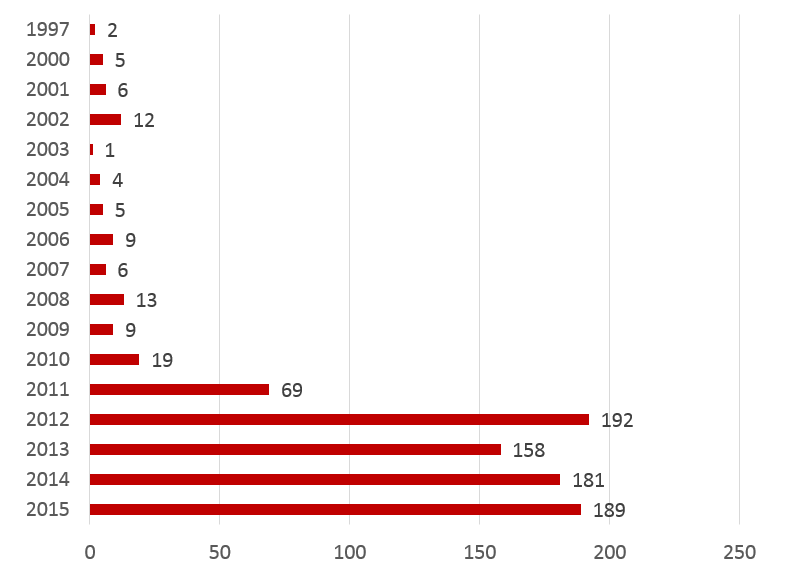
\includegraphics[width=14cm]{intro/PCSAttackEvent.png}
 \caption[fig:pcsattack]{1997-2015全球工业系统攻击事件.}
 \label{pcsattack}
\end{figure}


综上分析可以看出,不管是从网络信息安全还是从数据完整性的角度,PCS系统所面临的安全风险和入侵威胁都在不断增加,而且伴随着工业安全事故的数量逐年增加,相应带来的破坏和灾难也越发严重。所以,PCS系统的网络信息安全和数据安全已经成为越来越需要全面和深入研究的国家基础设施和关键领域。
正是在这种背景下,为了检测对PCS系统的入侵威胁,建立安全系统和关键国家基础设施安全的综合防御系统,本文重点谈久了基于PCS系统的入侵检测这样一个重要课题。

本文首先提出了对PLC的错误序列注入攻击,通过监视并控制PLC和实际物理设备之间的部分受感染传感器和足够的输出信号序列构造特定破坏序列注入到测量输入信号中。值得注意的是,在现有故障检测的条件下,我们利用容错率构造的攻击可以很好的绕开故障检测和诊断机制。根据控制系统不同层面的攻击特点,本文设计了一个双层检测和防御结构,以更好地保护SCADA系统。第一层主要是基于规范的程序攻击检测来应对网络侵入并攻击控制网络的情况,只有被检测并指示安全的程序和指令才能下载到可编程控制器设备中。基于第一层检测机制,我们可以保证运行在控制系统的程序的完备性和有效性,进而可以对控制器采集信号数据库,以执行第二层基于异常的数据完整性攻击检测。值得注意的是,我们创造性地提出了防御新型的控制器错误数据注入攻击尤其是错误序列注入攻击的检测和诊断方法,这是传统异常检测机制无法完成的工作。通过这两层检测,我们将为PCS系统构建一个完整的安全系统。

\section{过程控制系统与传统IT网络安全区别}


在过去,PCS使用专有硬件和软件,他们之间互连主要集中在总线通信。在20世纪90年代中期,人们将以太网和Microsoft Windows引入PCS,随后开发OPC接口,大大简化了本地与远程以及分布式通信问题,为此PCS也付出了暴露于以前仅为IT系统所知的安全威胁为代价。

此外,随着对工业系统的攻击在过去几年中迅速增加,企业的信息安全部门通常负责整个工厂的网络安全,包括其PCS。不幸的是,并不是所有的IT安全解决方案都适合PCS,因为PCS和IT系统之间存在根本的区别。此外,工业生产通常具有多个生产过程和PCS,并且一些工业生产过程自然比其他生产过程更关键。因此,在工厂中的各种PCS之间处理不同的安全性并不罕见。

虽然IT安全的良好剂量对工业控制系统安全至关重要,但是成功地保护控制系统需要额外的机制。工业控制系统的独特之处在于它需要将安全措施与大多数IT系统区分开来,其中一些因素包括控制系统放置在车间,而不是数据控制中心;它们存在置于危险环境或接近危险环境的风险;而且设备在平台上的平均寿命是在几十年而不是几年来衡量的也是不争的事实。

参考Belden工业以太网基础设施设计研讨会的信息,IT和PCS安全解决方案之间的差异有如下几个方面:
\begin{itemize}
	\item 性能要求
	\item 可靠性要求
	\item 操作系统和应用程序
	\item 风险管理目标
	\item 安全架构
	\item 安全目标
\end{itemize}

安全目标是两者之间的本质区别。例如,IT安全的第一目标集中于隐私,即保护数据;而PCS安全的第一目标是基于安全性,即保护该过程。

根据PCS本身特点,我们队其安全要求的问题又细分为三大类。这些问题是:

软目标:根据Belden,控制网络充满了所谓的“软”目标,即设备易受到网络接口干扰。许多工厂中的PC运行数周或数月,没有任何安全更新,有些甚至没有任何防病毒工具。此外,这些网络中的许多控制器是在网络安全不受关注的时代设计的,结果这些设备中的许多可能由于畸形的网络流量或甚至大量的正常流量而中断。

多路径:许多控制网络具有多种传输途径,网络安全威胁可以通过这些途径进入工厂。这些路径通常绕过工厂中的现有安全措施,有些甚至不出现在网络图上。例如,携带进出设施的笔记本电脑,或从一个PC移动到另一个PC的USB密钥。这些可以很容易地将恶意软件带入工厂,并迅速从一个系统传播到另一个系统。

平面网络:许多PCS网络仍然被实现为不相关子系统之间没有隔离的大且“平坦”网络。这意味着如果在设备中一部分出现问题,它可以非常快地传播到其他不相关的子系统,甚至到远程工厂站点。

根据参考文献[gervais12],对于PCS网络和IT网络的不同总结如下表\ref{intro:diffBetweenPCSandIT}
\newcommand{\tabincell}[2]{\begin{tabular}{@{}#1@{}}#2\end{tabular}}  
\begin{table}[!htp]
\centering
\caption{PCS与IT系统网络的区别}
\label{intro:diffBetweenPCSandIT}
\begin{tabular}{|p{2cm}|p{6cm}|p{6cm}|}
\hline
分类 & PCS系统 & IT系统 \\
\hline
优先级 & SRA(安全性,可靠性,可用性)是满足生产要求的最重要的特性。此外,发送到PLC的参数的完整性也是重要的。 & CIA(机密性,完整性,可用性)是IT中的优先考虑的安全因素。 \\
\hline
意识差异 & PCS工程师通常不能正确地解释恶意攻击者的能力。他们经常假设任何规范不允许的事情是不可能发生的。 & IT系统工程师认为如果攻击者能够获得对设备的物理访问,则很难保护它。 \\
\hline
风险管理 & 安全是主要关注的问题,即使安全问题可能会使安全受到威胁。 & 安全开始成为设计过程的组成部分。 \\
\hline
安全架构优先级 & 终端设备(如PLC)需要防止恶意攻击者。 & 数据资料需要保护。 \\
\hline
寿命 & 10-20年。 IT和PCS的融合可能会改变这个生命周期。 & 3-5年。 \\
\hline
实时要求 & 自动化设备具有严格的实时要求,因此需要满足最后期限。 & 通常没有严格的实时要求。 \\
\hline
物理交互 & 与设备,工作人员和生产过程的重要物理交互。 & 与环境的少量物理交互。 \\
\hline
资源约束 & 终端设备(PLC)具有有限的处理能力。 然而,近年来的设备的处理能力显着增加。 & IT系统通常具有重要和高效的处理能力。 \\
\hline
补丁管理 & 更新补丁很困难,因为可用性要求 需要开发定制解决方案。 & 补丁管理现在是一个标准过程。 静默更新在后台执行安装。 \\
\hline
供应商设备支持 & 通常需要原始供应商的支持。 & 支持来自各种来源的软件供应商。 \\
\hline
有限的物理访问组件 & 分布式系统使得对设备的访问困难且昂贵。 & 可以访问大多数IT系统。\\
\hline
\end{tabular}
\end{table}


\section{国内外研究现状}

\subsection{过程控制系统现存的攻击威胁}

传统过程控制系统受到的攻击计算机和网络威胁,例如内存侵入,目的是损害其一个或多个组件,以获得对系统行为的控制或者访问与进程相关的敏感数据。这里我们回顾近年来三类PCS漏洞的研究,第一类总体上研究PCS系统及其运营商的安全现状,第二类考虑PLC中的安全漏洞,第三类考虑传感器中的漏洞,在这种情况更侧重于智能电表,因为其是智能电网基础设施的重要组成部分。 

\begin{enumerate}
\item PCS总体安全现状:现有的研究[68]表明目前的PCS安全防护是有很大改进空间的。首先,因为PCS一直以来与因特网隔离并采用专有系统,所以经常被认为有很高安全性。然而,使用商用操作系统(例如,Microsoft Windows操作系统)和开放的标准网络协议使PCS不仅对于恶意攻击而且对因特网恶意软件的侵入感染都是开放的。例如,发生在俄亥俄州核发电站大面积破坏事件便是由于一些发电设施受到蠕虫病毒感染引起的。在10年内对100多个真实世界PCS进行渗透测试研究表明,在大多数情况下,这些PCS至少比标准补丁更新周期晚了一年。在某些情况下,将PCS与外部网络之间的DMZ隔离区域如果在几年内都没有更新的话,DoS攻击会变得很微弱。例如,在他们对网络连接的PLC的评估中,发现具有6字节分组的洪水攻击足以使PLC变得不可操作,导致所有状态丢失并迫使其重新启动。提高ICS安全性的另一个障碍是以下三个常见的错误[70]:
\begin{itemize}
\item 认为安全性可以通过隔离实现; 
\item 盲目部署安全技术提高安全性,例如防火墙、加密和防病毒软件的应用经常使系统操作者产生虚假的安全感;
\item 认为标准合规性可以保证系统安全,事实上即使北美能源可靠性公司提出的网络基础设施保护标准[71]也被批评为提供虚假的安全感[72]。 
\end{itemize}
\item 对PLC的攻击:PLC监视和操纵物理系统的状态,最常用的西门子PLC也被证明有漏洞。由于缺乏适当的会话饱满度,这些PLC使用的ISO-TSAP协议可以实现重放攻击[73],也可以绕过PLC认证上传有效载荷,并在PLC上执行任意命令。有研究表明用于监狱设施的西门子PLC也存在被操纵监狱门的可能性[74]。 
\item 对传感器的攻击:PCS的另一个关键组成单元是收集数据并将其传送回控制单元的传感器。智能电表作为演进智能电网的广泛部署的要素具有与传统模拟电表相同的形状因子[75]和多个增强特征:使用时间定价[76]、自动读表、电力质量监视和远程电源断开。现实世界智能计量系统的安全评估通常被认为是通过篡改测量值引发类似能源盗窃等一系列安全事故[77]。存在研究表明受测系统在被实施重放攻击时允许在在仪表的内存以及飞行中进行不可检测的篡改测量值操作。后续研究检查了来自多个供应商的计量表时发现允许针对任意仪表的DOS(拒绝服务)攻击的漏洞,而且可以对远程断开开关进行完全控制使得能够有目标地断开对客户的服务[78]。
\end{enumerate}

除了上述总结的传统安全威胁,这里我们着重考察PCS攻击的两个新方向。其中第一类构造了针对对手可能不具有完全访问权的PCS的程序篡改攻击。第二类攻击操纵传感器输入以误导控制系统尤其是可编程控制器执行动作。 
\begin{enumerate}
\item 程序篡改攻击:一种类型的攻击旨在收集有关受害者PCS的情报。例如,Duqu蠕虫病毒主要收集关于受害者系统的信息[79],然后将其转发到命令和控制服务器。对PCS的另一种类型的攻击旨在影响受害者系统的物理行为,这种攻击的最着名的例子是Stuxnet蠕虫,其攻击手段主要是操纵用于铀浓缩的一组离心机的参数。这样的攻击有两个阶段:感染和上传恶意程序。传统来说一旦攻击者破坏了信息系统,上传预先构建的恶意程序是不难的。这是因为攻击者通常有一个被攻击的软件的副本。然而对于PCS则不一定是这种情况,根据攻击者实施的攻击类型,恶意程序的构造可能容易出错或几乎不可能。恶意程序是无区别的或有针对性的,不加区分的恶意程序执行随机攻击,在受害者PCS的机制内引起恶意行为。有几种方式恶意软件可以在获得对一个或多个受害者PCS PLC的访问时自动构造不加区分的有效载荷[80]。这里的假设是,如果恶意软件能够写入PLC代码区域,则它还必须能够从PLC代码区域进行读取。由于具有读取PLC代码的能力,首先恶意软件推断出被称为互锁的基本安全属性[82],并生成一个恶意程序,其可以违反尽可能多的安全属性。 其次恶意软件识别系统中的主定时环路。考虑交通灯的示例,其中主循环确保每种颜色的光在特定时间段内依次有效。然后,恶意软件可以构造违反定时循环的恶意程序,例如通过允许某些光重叠。 最后在总线枚举技术中,恶意软件使用标准化标识符(如现场总线ID)来找到受害系统中的特定设备[83]。
\item 错误数据注入(FDI)攻击:在FDI攻击中,攻击者选择一组注入到一个或多个控制器的传感器,然后向这些传感器提供精心制作的恶意值,从而使控制器获得预期的结果。例如,如果所提供的恶意值告诉控制器温度变得太低,则它将令加热元件不断增加温度,即使实际温度很好也会导致未检测到的设备过热。最早的FDI攻击目标是电力系统状态估计[85]。状态估计是分布式控制系统中的重要步骤,其中基于多个可观测量来估计实际物理状态。电力系统状态估计确定电力负载如何分布在输电网络中的各种高压线路和变电站上。人为干扰相量测量单元(PMU)的子集可导致不正确的状态估计。[86]报道了基于卡尔曼滤波的状态估计的FDI攻击。卡尔曼滤波器是比线性和直流系统模型更一般的状态估计形式,基于卡尔曼滤波器的状态估计器对FDI攻击的敏感性取决于设计系统的固有属性[86]。如果基础状态转移矩阵包含不稳定的特征值,则系统只保证通过FDI攻击是可控的。这不仅对攻击具有重要的意义,而且对于针对FDI攻击的防御具有重要的意义,因为缺乏不稳定特征值的系统可能不会被完全攻击。

\end{enumerate}




\subsection{}

\section{论文组织结构}


%# -*- coding: utf-8-unix -*-
%%==================================================
%% chapter02.tex for SJTU Master Thesis
%% based on CASthesis
%% modified by wei.jianwen@gmail.com
%% Encoding: UTF-8
%%==================================================

\chapter{过程控制系统的错误序列注入攻击}
\label{chap:FSIattack}

\section{引言}
\label{sec:intro}

过程控制系统作为国家关键基础设施的基本组成部分已经广泛应用于工业和物联网系统中。正因为它们在现代工业社会中的关键作用,使得它们成为怀有恶意目的的攻击者的感染和侵袭的目标。传统的安全保护主要是通过多层网络防火墙和成熟的的病毒防御软件阻止网络攻击入侵工业网络。然而考虑到网络和复杂的硬件系统实施,这些方法不能完全保护网络和硬件平台免受不断变异的威胁侵入,例如Stuxnet病毒侵入人机界面(HMI)服务器并上传恶意代码到可编程逻辑控制器PLC使其损坏制造核原料的离心机。考虑到HMI服务器通常安放在在受良好保护的工业控制网络中,所以对其实施攻击是非常困难的。

本章我们提出的错误序列注入(FSI)攻击,可以通过感染和篡改PLC的输入信号迫使其执行误操作和破坏控制系统的关键设备。因为PLC的输入仅仅来自假设被FSI攻击注入的远程传感器,所以在不需要渗透到防御坚固的控制网络并执行恶意代码上传的情况下便可以对系统实施有目的性攻击。值得注意的是我们构造的攻击可以避开现有的系统故障检测机制,并利用其容错率漏洞来构造基于离散时间模型的FSI攻击。

\section{攻击模型概述}
\label{sec:formulation}

考虑到图1描述的威胁模型,攻击者只需要侵入并控制遍布在远程的信号采集传感器。从过去的假数据注入攻击研究[5],[9],[19],[20],[30]中我们知道大部分工业控制系统包括电力系统的远程传感器如相量测量单元在实践中受到的保护较少并且分布在全国各地,因此与控制网络内的服务器相比更容易访问和侵入。我们假设攻击者知道高级基础设施配置,即连接到PLC传感器和执行器的输入输出的变量映射关系,这样攻击者不必渗透到控制网络中FSI攻击仍然可以成功。即使HMI服务器没有泄密而且攻击者也没有获得在PLC设备上上传恶意控制器程序的权限,我们构造的错误序列攻击只需要注入并控制向PLC发送测量信号的传感器便可以对控制系统造成不可逆的破坏。

\begin{figure}[!htb]
  \centering
  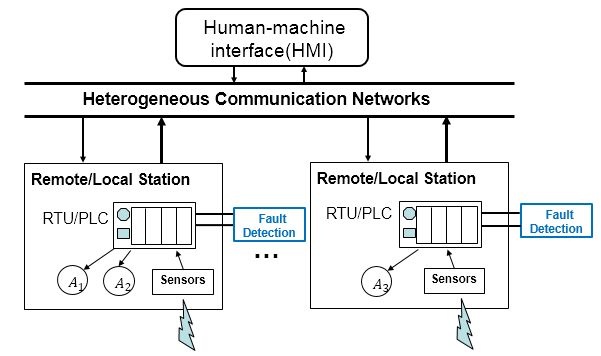
\includegraphics[scale=0.45]{att/threatModel1.png}
  \caption{FSI攻击威胁模型}
  \label{fig1}
\end{figure}

然而困难是如何在现有控制系统中部署的成熟故障检测的情况下构建攻击使PLC执行误动作。FSI攻击的主要任务之一是分析并且绕开故障检测机制。通常来看用辨识精度不高的系统模型来检测随机性的故障能够得到很高的准确度,我们通过这一特性反向构造错误序列并且注入到受控制的远程传感器则可以达到使故障检测失效的目的。图\ref {fig2}显示了攻击是如何构造的。我们假设对手可以访问在PLC控制器和物理设备之间交换的信号或堆栈数据。然后利用输入和输出向量数据库,我们辨识出与故障检测的建模方法类似的无故障的离散事件模型。最后,我们搜索所有的不可被故障机制检测的虚假序列的集合,并且获得适当长度的恶意序列对受控制的传感器采集的输入信号进行篡改。

\begin{figure}[!htb]
  \centering
  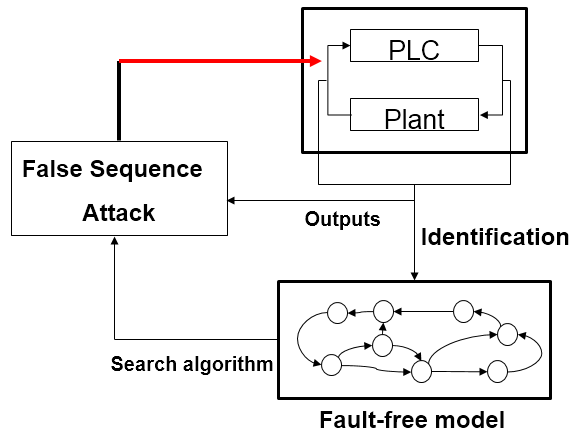
\includegraphics[scale=0.45]{att/ASC2.png}
  \caption{FSI攻击构造示意图}
  \label{fig2}
\end{figure}

\section{系统建模和攻击构造}
\label{sec:model}

我们需要一个形式化的描述来辨识特征值为$m$的系统模型$ \textbf{BEH}_{Ident}^m $和观测信号模型\( \textbf{BEH}_{Obs}^m \),从形式化模型定量生成特征值大于$m$特征向量。辨识的目标是使得在给定便是参数$k$的条件下特征值超出$k$的特征向量数目达到最小,理想情况是$ \textbf{BEH}_{Ident}^m $与$\textbf{BEH}_{Obs}^m $相等。最后我们在辨识得到的系统模型和观测信号模型基础上搜索FSI攻击序列。

\subsection{信号采集和观测特性定义}

我们通过在PLC控制器获取信号之后以固定时间间隔读取信号来采样数据\cite {roth2012}。图\ref {fig3}显示了从PLC采样$I/O$向量序列的最常用的方法,通过OPC通信模式收集在服务端接收到的$I/O$数据形成标识数据库。

\begin{figure}[!htb]
  \centering
  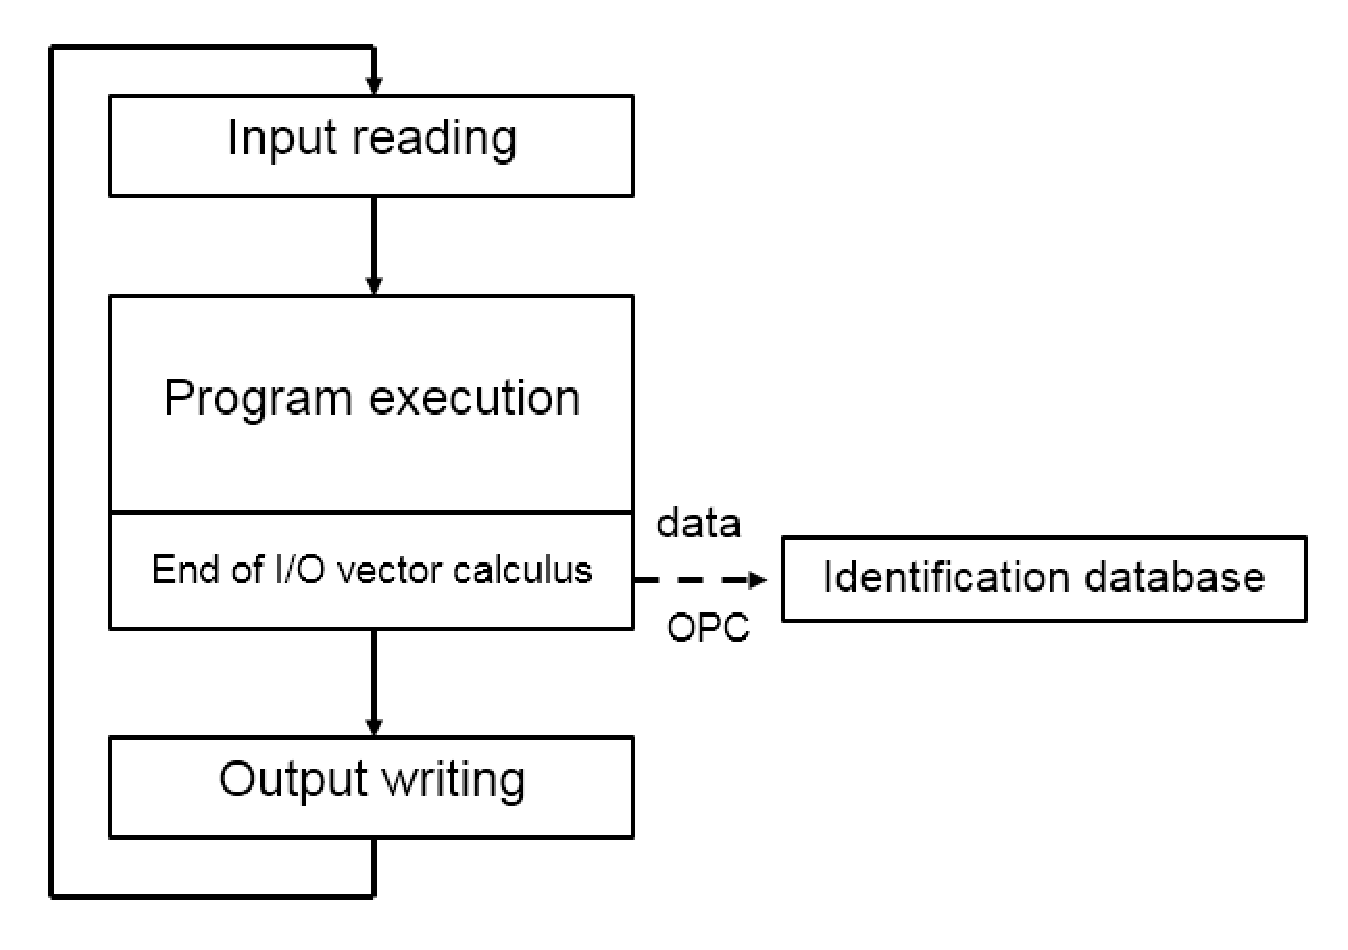
\includegraphics[scale=0.45]{att/database2.eps}
  \caption{对PLC采样数据示意图}
  \label{fig3}
\end{figure}

在实现数据收集之后,我们需要定义观察到的输入/输出($I/O$)序列、采样数据的语义和词义。 首先我们引入以下定义,

\textbf{定义1:} \( r \)个输入和$ s $ 个输出的采样数据的观测$I/O$序列集合定义为:

\begin{equation} 
\Sigma = (\gamma_1,...,\gamma_p) 
\end{equation} 这里 $\gamma_i = (u_i(1),u_i(2),...,u_i(|u_i|))$, $ u_i(j) $ 是第$i$个$I/O$向量$u$的第$j$个输出,其中$ u = (I_1,...,I_r,O_1,...,O_s) = (IO_1,...IO_m) $ 且 $ m=r+s $.

我们假设对于$ \forall $两个连续的$I/O$向量$ u(t)\ neq u(t + 1)$ 成立
当且仅当至少一个$I/O$向量分量改变且$I/O$向量是新生成的。

\textbf{定义2:} 观测到的采样数据词义集合表示和语义集合表示: 观测的词义可以用$I/O$序列长度为$q$的观测向量集合描述 
\[
L_{Obs}^q = \bigcup_{\gamma_i \in \Sigma} \Big(\bigcup_{t=1}^{|\gamma_i|-q+1} (u_i(t),u_i(t+1),...,u_i(t+q-1))\Big) 
\]

有了词义的形式化表示后,我们定义长度为$n$的采样数据的语义的表示:
\begin{equation}
 \textbf{BHE}_{Obs}^n = \bigcup_{i=1}^n L_{Obs}^i 
\end{equation}

\subsection{模型辨识}

\subsubsection{模型选择}

模型辨识的目的是确保辨识的任意长度为$ m $的语义表示$ \textbf {BEH}_{Ident}^m $等于观测到的任意长度为$ m $的语义表示  \( \textbf{BEH}_{Obs}^m \),其中$ m $可以是任何正整数。 简而言之,所辨识的模型在精度足够高的情况下能够完美复现基于PLC的过程控制系统。考虑到过程控制系统通常是可编程的控制器和物理设备的耦合系统,可编程的控制器可以被认为是确定性的,而物理设备通常被认为是非确定性的。因此,物理设备和控制器的耦合系统一定是非确定性的。因此,我们提出了适合于辨识过程控制系统的非确定性自发输出自动机(NDAAO)\parencite{klein2005}。

\textbf{定义3:} NDAAO是由5元组函数表示: \[ NDAAO=(X,\Omega,\textit{f}_{nd},\lambda,x_0) \] with\
\begin{itemize}
  \item $ X={x_0,...,x_{|x|-1}} $ 是有限状态集
  \item $ \Omega={\omega_1,...,\omega_{|\omega|}} $ 是有限输出变量集
  \item $ \textit{f}_{nd}: X\rightarrow 2^X $ 是非确定性转移函数
  \item $ \lambda: X\rightarrow \Omega $ 是状态对应的输出函数
  \item $x_0$ 是初始状态
\end{itemize}

NDAAO可以由图$G=(V,E)$的形式表示,图$G$的定点集是NDAAO所有的状态集,有向边集是由非确定性转移函数$f_{nd}$组成,即\[ E(G)=\big\{(x_i,x_j)\in X\times X: x_j\in f_{nd}(x_i)\big\} \],每个节点对应一个状态并包含状态对应的输出,图~\ref{fig4}通过一个简单的例子来展示图形化的NDAAO模型。

\begin{figure}[!htb]
  \centering
  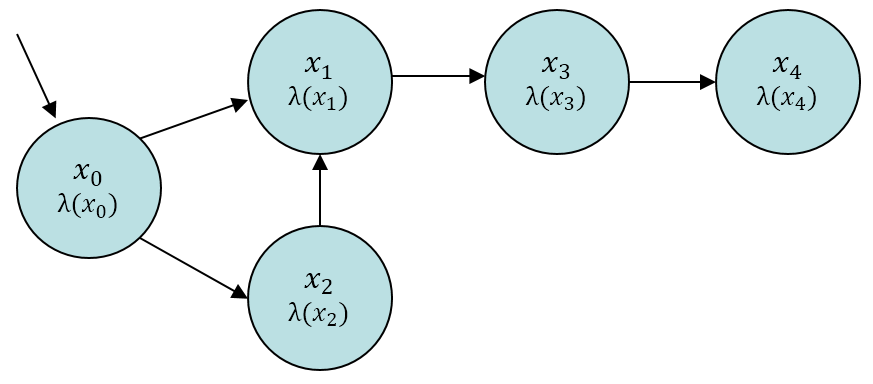
\includegraphics[scale=0.18]{att/ndaao_example.png}
  \caption{NDAAO图形表示}
  \label{fig4}
\end{figure}

\textbf{定义4:} NDAAO的词义和语义表示: 由开始状态为$x_i$NDAAO生成的长度为$n$词语集合表示为
\begin{equation} 
W_{x_i}^{n}=\left\{\begin{split} &w\in \Omega^n~|~ w=\big( \lambda(x(1),...,\lambda(x(n))) \big):\\ 
&[\exists \big(x(1),...,x(n)\big): x(1)=x_i\in X,~and\\
&\forall\;1\leq t\leq n-1, x(t+1)\in f_{nd}(x(t))] \end{split} \right\} 
\end{equation} 然后由词语组成的长度为$n$词组集合表示
\begin{equation} 
W^n(NDAAO)=\bigcup_{x_i\in X} W_{x_i}^{n} 
\end{equation} 有了词组集合,我们可以获得NDAAO的长度为$n$语义集合表示
\begin{equation} 
\textbf{BEH}_{Ident}^n=\bigcup_{p=1}^n W^{p}(NDAAO) 
\end{equation}

\textbf{定义5:}辨识事件向量$\varepsilon(j)$是NDAAO中相邻两个辨识输出向量$\omega(j)$ 和 $\omega(j+1)$ 的变化量,用公式表示为 $\varepsilon=\omega(j+1)-\omega(j)$. 输入事件向量 $I(\varepsilon(j))$ 是相邻两个辨识输入向量 $I(j)$ 和 $I(j+1)$的变化量,同理输出事件向量$O(\varepsilon(j))$也有相似的定义. 具体的公式表示为:
\begin{equation} 
\varepsilon(j)=\bigcup_{l=1}^m \begin{cases}
I_l\_1~or~O_l\_1,~if~ I_l(j+1)-I_l(j)=1\\
I_l\_0~or~O_l\_0,~if~ I_l(j+1)-I_l(j)=-1\\
\epsilon,~if~ I_l(j+1)-I_l(j)=0
\end{cases} 
\end{equation}

考虑包含两个输入和一个输出的$I/O$向量序列$\gamma$,我们得到 \[\gamma=(A,B,C)=( \begin{bmatrix}
0\\1\\0
\end{bmatrix},\begin{bmatrix}
1\\1\\0
\end{bmatrix},\begin{bmatrix}
1\\0\\1
\end{bmatrix})\]

该序列可以简化表示成 $A\xrightarrow{I_1\_1}B\xrightarrow{I_2\_0,O_1\_1}C\cong A\xrightarrow{I_1\_1,I_2\_0,O_1\_1}C$

\subsubsection{辨识算法}

本节我们提出了一个辨识算法用来生成上一节中所描述的NDAAO模型。我们定义辨识参数$ k $用于确定用于生成新状态的$I/O$向量序列的长度。如果生成的NDAAO模型的长度为$ k $的语义集合正好与观测时采样数据产生的长度为$k$的语义集合一致的话,这样的NDAAO模型被称为$ k $完全可观测的。

NDAAO的构造主要分为三个步骤。首先,我们将观察到的序列转换为一组长度为$ k $的词组序列并在每组的第一个状态前创建一组长度为$ k-1 $ 伪状态以确保与其他词语一致。算法1的第一部分表示了观测序列的转换过程。然后我们开始执行NDAAO辨识操作, 将NDAAO的状态集与长度为$ k $的词组集相关联,并且转移函数由长度为$ k+1 $的词语表示。算法\ref{algo:ndaao}的第二部分表示了NDAAO的辨识过程​​。最后,我们合并等效状态来对状态空间进行降维,对于任意两个不同的状态$ x_i $和$ x_j $,如果它们相关联的输出相同并且它们具有相同的后继状态集,则我们可以将这两个状态合并到一个状态。我们通过从NDAAO的状态集和转移函数绘制状态转移图来使模型可视化。具体过程如算法\ref{algo:graph}所示。

\begin{algorithm}[h]
  \caption{NDAAO构造算法}
  \label{algo:ndaao}
  \begin{algorithmic}[1]
    \Require %算法的输入参数:Input
    观测的$I/O$序列(采样数据) $\varSigma$ 和辨识参数 $k$
    \Ensure %算法的输出:Output
    NDAAO模型和状态转移图 $G=(V,E)$;  \\
    // \textbf{第一部分:观测序列的转换过程}
    \For{each $\gamma_i \in \varSigma$}
      \If {$u_i(1)\neq u_i(|\gamma_i|)$}
          \State  从$\varSigma$删除$\gamma_i$; Return;\
        \Else
        \State $\alpha_i(t)=\begin{cases}
        u_i(1),\quad for ~~ 1\leq t\leq k-1\\
        u_i(t-k+1),\quad for ~~ k \leq t \leq k+|\gamma_i|-1
        \end{cases}$\
        \For {$m=1~~to~~|\gamma_i|$}
        \State $w_i(m)=(\alpha_i(m),...,\alpha_i(m+k-1))$;
        \EndFor
        \State $\gamma_i^k=(w_i(1),...,w_i(|\gamma_i|))$;
        \EndIf
    \EndFor
    \State $\varSigma^k=\bigcup\limits_{i=1}^{|\varSigma|}  \gamma_i^k$;\\
    \State \textbf{第二部分:NDAAO的辨识过程​​}初始化状态集 $X=\emptyset$, 转移函数 $f_{nd}(x_0)=\emptyset$, 输出 $\Omega=\emptyset$, 初值状态 $x_0=\varSigma^k[0][0]$, 节点集 $N=\emptyset$ 和边集 $E=\emptyset$;
    \ForAll {$\xi$ such that $\xi \in \varSigma^k$} 
      \ForAll {$\eta$ such that $\eta \in \xi$}
      \State $X\leftarrow X\cup \xi$; $\Omega \leftarrow\ \Omega \cup \eta(|\eta|)$;
      \EndFor
    \EndFor
    \ForAll {$\delta$ such that $\delta \in \varSigma^{k+1}$} 
      \ForAll {$\psi$ such that $\psi \in \delta$}
      \State $x \leftarrow \psi[1-k]$;$f_{nd}(x)=\psi[k-|\psi|]$;  
      \EndFor
    \EndFor
  \end{algorithmic}
\end{algorithm}

\begin{algorithm}[h]
  \caption{状态空间降维和图形化表示}
  \label{algo:graph}
   \begin{algorithmic}[1]
\ForAll {$x_i,x_j$ such that $x_i,x_j \in X and i\neq j$}
      \If {$\lambda(x_i)=\lambda(x_j)$ 和 $f_{nd}(x_i)=f_{nd}(x_j)$}
        \State 合并 $x_i$ 和 $x_j$, 从$X$中删除 $x_i(x_j)$ 并且用$f_{nd}(x_{pre})=x_j(x_i)$替换$f_{nd}(x)=x_i(x_j)$, 这里$x_{pre}$是$x_i(x_j)$的前继;  
      \EndIf
    \EndFor
    \State $V\leftarrow\ V\cup X$;
    \State $E \leftarrow E\cup (x,f_{nd}(x))$;
    \State 对$G(V,E)$画图;
  \end{algorithmic}
\end{algorithm}
\textbf{例子1.} 考虑从无故障例子系统中采样三组向量序列: $\gamma_1=(A,B,C,D,E,A)$, $\gamma_2=(A,B,D,C,D,E,A)$, $\gamma_3=(A,D,B,C,D,F,E,A)$. 大写字母代表不同的$I/O$向量。这里我们选取辨识参数$k=2$,经过序列转换后我们得到 \[\begin{split} \gamma_1^{k=2}&=(AA,AB,BC,CD,DE,EA)\\ \gamma_2^{k=2}&=(AA,AB,BD,DC,CD,DE,EA)\\\gamma_3^{k=2}&=(AA,AD,DB,BC,CD,DF,FE,EA) \end{split}\] 和 \[\begin{split} \gamma_1^{k=3}&=(AAA,AAB,ABC,BCD,CDE,DEA)\\ \gamma_2^{k=3}&=(AAA,AAB,ABD,BDC,DCD,CDE,DEA)\\\gamma_3^{k=3}&=(AAA,AAD,ADB,DBC,BCD,CDF,\\&\quad \ DFE,FEA) \end{split}\]

在获得$\Sigma^{k=2}$ 和 $\Sigma^{k=3}$之后,我们从$\Sigma^{k=2}$得到状态集并且通过算法\ref{algo:ndaao}的第二部分从$\Sigma^{k=3}$得到转移函数。相应的例子示意如图~\ref{fig5}所示。

\begin{figure}[!htb]
  \centering
  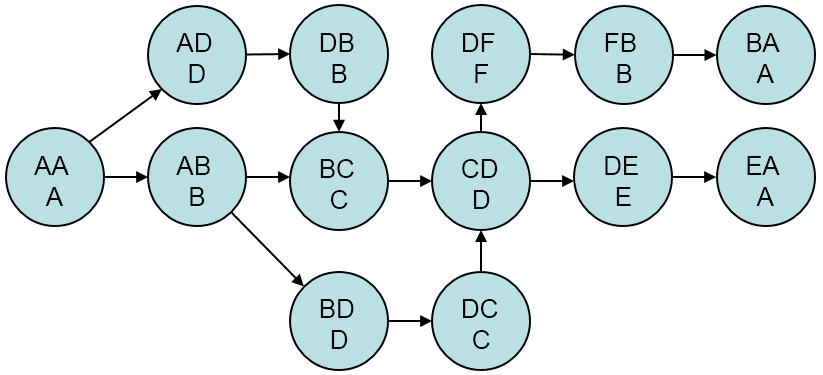
\includegraphics[scale=0.44]{att/2dot_graph.png}
  \caption{经过两步辨识算法得到的NDAAAO模型图示}
  \label{fig5}
\end{figure}

初始辨识的模型相比真实系统存在冗余的状态集和边集,因此需要根据算法\ref{algo:ndaao}的第三部分来减少状态空间以简化初始模型。在例1中如果我们将状态$ DB $与状态$ AB $、状态$ BA $与状态$ EA $、状态$ BC $与状态$ DC $均合并,并且对任意$x_i \in X$用$x_i$替换长度为$k$的向量词语。我们得到的简化NDAAO模型如图~\ref{fig6}所示.

\begin{figure}[!htb]{}
  \centering
  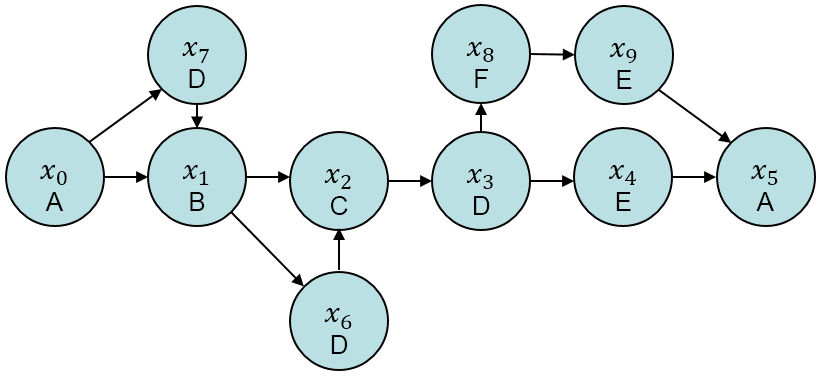
\includegraphics[scale=0.24]{att/3dot_graph.png}
  \caption{最终简化的NDAAO模型图示}
  \label{fig6}
\end{figure}

\subsection{FSI攻击的构造}

在我们辨识出无故障的NDAAO之后,我们可以利用故障检测的原理构造不可检测的错误序列。我们知道,故障检测是根据当前观测的$I/O$向量与辨识的NDAAO的预期输出是否一致来确定是否存在故障的。如果结果为真,则认为当前观测向量安全,否则给出警报可能存在故障。在我们的攻击方法中,我们构造了错误序列注入攻击,其不仅满足序列输出来自辨识的模型以确保不能被故障机制检测到,而且还通过选择具有恶意执行逻辑的适当长度的错误序列注入到控制器的输入信号中来破坏系统。从$ x_i $开始的长度为$ n $的错误序列的具体形式描述如下定义,
\begin{equation} 
S_{x_i}^{n}=\left\{\begin{split} &s\in \Omega^n~|~s=\big( \lambda(x(1),...,\lambda(x(n))) \big)\wedge\\
&(s\notin L_{Obs}^n):[\exists \big(x(1),...,x(n)\big): x(1)\\&=x_i\in X,~and~
\forall\;1\leq t\leq n-1,\\&x(t+1)\in f_{nd}(x(t))] \end{split} \right\} 
\end{equation}

上述定义的$ S_{x_i}^{n} $从辨识的NDAAO模型中截取长度为$ n $的序列并且不同于观测到的$I/O$向量集的任何长度为$ n $的序列。因此,定义的错误序列当注入到控制器的输入信号时能够对控制系统造成潜在的入侵破坏。由于降维的NDAAO是$(k + 1)$完全可观测,故以下等式成立:
\begin{equation} 
\forall~m\leq k+1,~~\textbf{BEH}_{Obs}^m=\textbf{BEH}_{Ident}^m 
\end{equation}

根据上述理论,只有当$ S_ {x_i} ^ {n} $中长度不小于$ k-2 $的序列才可以是错误序列。我们基于辨识参数$ k $ 获得从NDAAO生成的所有错误序列集合为
\begin{equation} 
A^k=\bigcup_{x_i\in X} \big( \bigcup_{n=k+2}^{max(|\gamma_d|)} (S_{x_i}^{n})\big),~\gamma_d\in \Sigma \end{equation}

在我们得到错误序列的定义之后,下一步是提出搜索算法以获得所有不可被故障机制检测的错误序列集合。从算法\ref{algo:fsi}可以看出使用FSI递归遍历算法的递归公式可以获得长度不小于$ k + 2 $的错误序列,这些序列来自于NDAAO模型选择且不存在于开始状态为$ x_ {init} $的观测$I/O$向量的序列的任意子序列。通过获取FSI递归遍历算法的输出,我们合并所有$ X $中始于状态$ x_ {init} $的$ S_ {x_ {init}} $的序列集合$ A ^ k $,具体表达式如下,
\begin{equation} 
A^k=\bigcup_{x_{init}\in X} \big(S_{x_{init}}\big) 
\end{equation}


\begin{algorithm}[h]
  \caption{FSI递归遍历算法}
  \label{algo:fsi}
  \begin{algorithmic}[1]
    \Require %算法的输入参数:Input  
    辨识的NDAAO模型, 观测的$I/O$序列 $\varSigma$, 辨识参数 $k$ 和初始状态 $x_{init}$ \\  
    
    \Ensure %算法的输出:Output  
    错误序列集合 $S_{x_{init}}$;  \\
    \For{each $x \in x_{init}$}
      \State $x_{init}=f_{nd}(x)$
      \State $seq$.append$(x)$
      \State $IncSearching(NDAAO,\varSigma,k,x_{init})$
      \If {$|seq|\geq (k+2)$ and $ seq\notin substring(\gamma) ~for~\forall\gamma\in\varSigma$}
        \State $S_{x_{init}}$.append$(seq)$
      \EndIf
      \State $seq$.pop()
    \EndFor
    \State Return $S_{x_{init}}$
  \end{algorithmic}
\end{algorithm}

通过算法\ref{algo:fsi},获得的示例1的错误序列的集合是${(A,D,B,D,...),(...,D,C,D,F,...),(A,B,C,D,F,...)}$,其中字母之前或之后的省略号可以是字母的任何前导或后继。

因为攻击者可能对来自控制系统的传感器的控制有限,我们需要确定在从上述方法产生的错误序列的两个连续向量之间变化的$I/O$向量分量。

\subsection{可行性和性能指标}

本文攻击的可行性主要来自两方面。 首先随着辨识参数$ k $的增加,NDAAO的状态空间迅速增加并且需要采样庞大的顺序系统进程周期信号数据才能使模型收敛到稳定水平\parencite{klein2005}。因此,当在精度值$ k $较大的条件下进行在线检测时往往需要大量的计算。 我们的工作主要实现离线攻击,有足够的时间进行计算。其次,考虑到检测机制的稳定性和性能,在实际工业系统中通常一个较小的参数$ k $足以满足基于故障检测的实际要求\parencite{roth2012},也正是因为这两个条件,较小的参数$ k $能够为我们的攻击的构造提供良好的可行性。

为了评估NDAAO的连通性,我们给出由一个状态产生的后继边的平均数量的信息。 我们定义结构复杂度指标$ C_s $ 如下:
\begin{equation}
C_s= \dfrac{\sum_{x_i\in X} (deg(x_i))}{|X|} 
\end{equation} here $deg(x_i)=|f_{nd}(x_i)|$ is the degree of a state.

与复杂性指标类似,我们定义攻击脆弱度指数来衡量从已辨识的NDAAO模型中搜索错误序列的成功率。攻击脆弱度指数定义如下所示:
\begin{equation}
 C_A^n=\dfrac{|\bigcup_{x_i \in X}(A_{x_i}^n)|}{|W_{Ident}^n|} 
 \end{equation}

通过方程(11)和(12),我们可以获得所有状态的多重分支状态的比率和所有辨识的$I/O$序列集中错误序列的比率。
\section{实验仿真}
\label{sec:simulation}

为了证明所提出的错误序列攻击方法的可行性和性能,我们给出了相应的案例仿真。 考虑的系统是一个小型的货物分拣系统,该系统的功能是根据尺寸大小分拣包裹。系统有11个输入(来自物理设备的输出信号)和5个输出(从PLC输入到物理设备的信号)。 图\ref{fig7}显示了货物分拣系统的结构示图。
\begin{figure}[!htb]
  \centering
  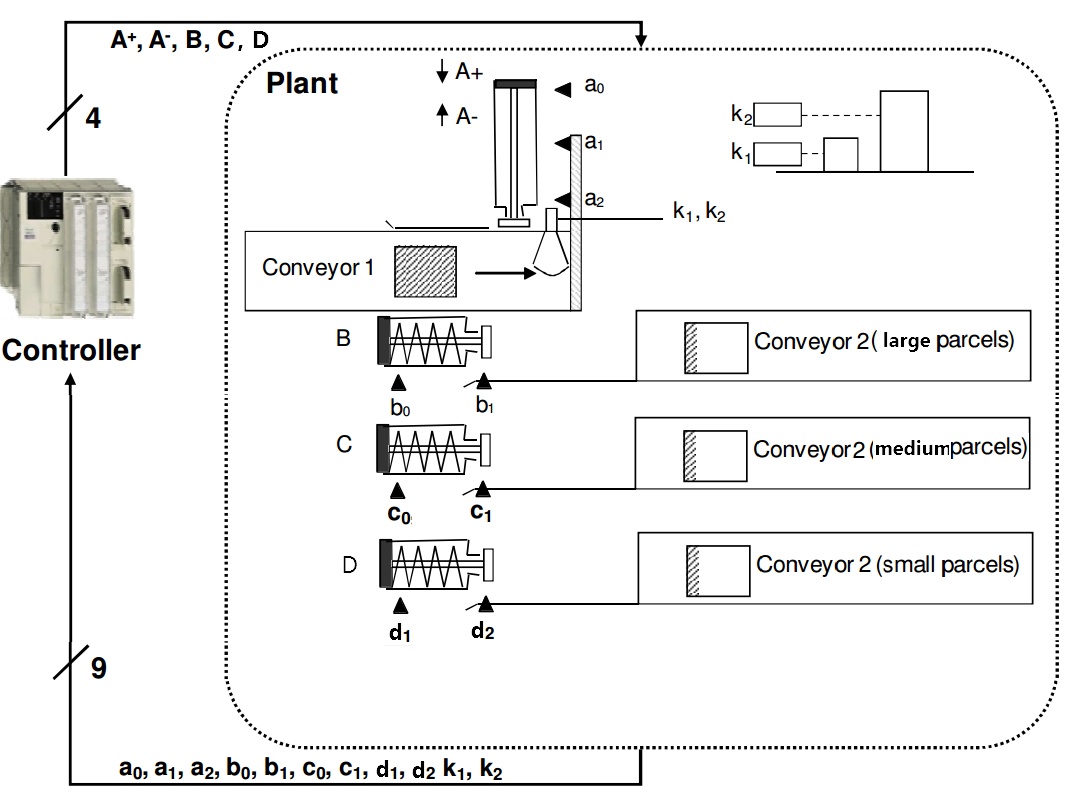
\includegraphics[scale=0.48]{att/sort.png}
  \caption{货物分拣系统的结构示图}
  \label{fig7}
\end{figure}

\begin{figure}[!htb]
  \centering
  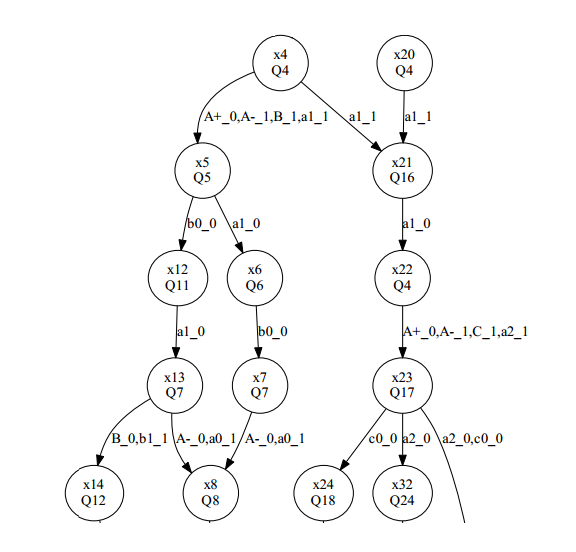
\includegraphics[scale=0.31]{att/casendaao.png}
  \caption{货物分拣系统的部分NDAAO模型}
  \label{fig8}
\end{figure}


辨识数据库是由50个采样的系统运行周期组成并且每个周期的采样时间均为货物到来和分拣时刻。系统的输入和输出变量向量为$[A+,A-,B,C,D,k_1,k_2,a_0,a_1,a_2,b_0,b_1,c_0,c_1,d_0,d_1]$。在完成辨识过程和状态空间降维后,我们得到货物分拣系统完整的NDAAO模型,由于篇幅所限部分模型如图\ref{fig8}所示。
\begin{figure}[!htb]
  \centering
  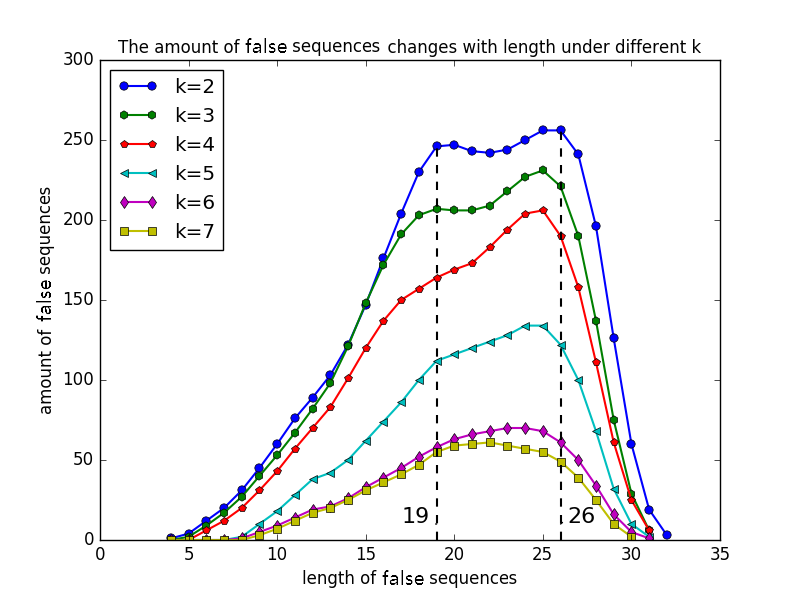
\includegraphics[scale=0.29]{att/length.png}
  \caption{不同数量的错误序列数量}
  \label{fig9}
\end{figure}

\begin{figure}[!htb]
  \centering
  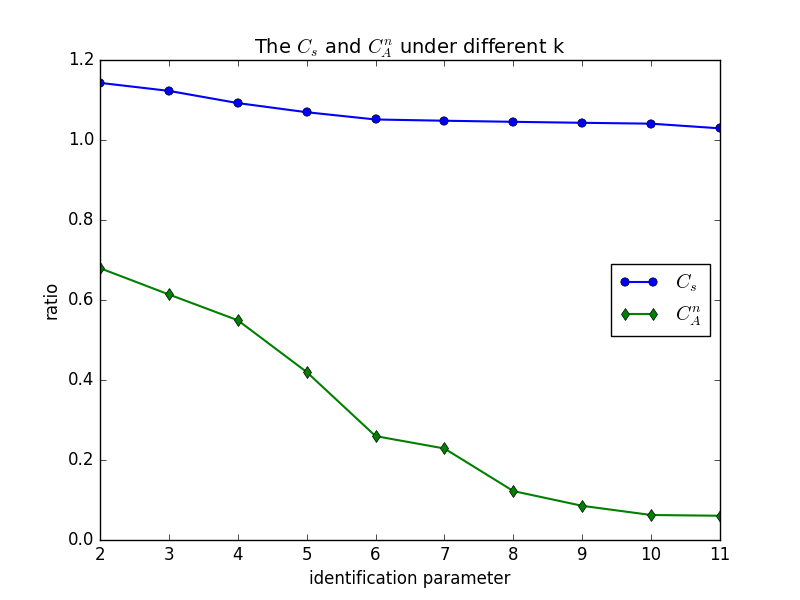
\includegraphics[scale=0.39]{att/vuln.png}
  \caption{$C_s$ 的 $C_A^n$关系}
  \label{fig10}
\end{figure}

通过获得的模型,我们执行了错误序列搜索过程,在简化之前我们搜索了大量不同长度的假序列,这些错误序列可以作为潜在的恶意逻辑顺序注入到受控传感器中。例如\[\begin{split} A_1&=Q_{34}Q_{21}Q_{22}Q_{30}\\A_2&=Q_{32}Q_{10}Q_{11}Q_{12}Q_{28}\\A_3&=Q_{16}Q_{17}Q_{18}Q_{19}Q_{20}Q_{34} \end{split}\],这里$Q_i$是每个观测周期的输出向量。\\

然而如果攻击者实施攻击,必须需要保证上述序列所有的传感器受到感染和控制,这在实际操作中是很难实现的。因此我们需要使用来自等式(6)的驱动事件向量简化处理如上所述在序列集,结果如下:\[\begin{split} A_1&=Q_{34}\xrightarrow{d1\_1,b0\_1,\{b0\_0,d0\_1\}}Q_{30}\\A_2&=Q_{32}\xrightarrow{d1\_1,b1\_1,k2\_1,\{b1\_0,d0\_1\}}Q_{28}\\A_3&=Q_{16}\xrightarrow{\{k1\_0,a0\_0,c1\_1d1\_0\},a1\_1,a1\_0,k2\_1,\{a2\_1,c1\_0\}}Q_{34} \end{split}\],这里,用逗号分隔的每个箭头的符号序列是在错误序列的每两个向量之间的单个驱动事件输入的集合。当我们注入这些错误序列到PLC控制器的输入信号时,在没有被故障机制所检测的情况下,分拣结束后将获得错误的分拣结果。
从获得的假序列,我们发现大多数假序列集中在19和26之间的长度。所以潜在的恶意攻击可以选择这种长度的假序列。图。\ref{fig9}显示了不同$ k $下假序列变化的长度。
考虑到良好的攻击可行性需要较大的状态度和较多的多分支状态,图\ref{fig10}显示了在结构复杂度度量$ C_s $(多分支状态的比率)减小的情况下,攻击脆弱度指数(错误序列的占比)快速下降。因此我们可以通过在多个分支状态上添加特定的检测机制来避免这种攻击,而不是一味地提高辨识参数$ k $。

\section{本章小结}

在本章中,我们基于过程控制系统提出了一种错误序列注入攻击,所获得的错误序列攻击将被用作注入到与PLC连接的远程传感器接收的信号来对系统进行恶意逻辑攻击。我们给出了包括FSI递归搜索算法在内的错误序列注入攻击构建的整个实现过程。值得注意的是对多个分支状态的检测将成为对这种攻击的有效防御。实验仿真表明我们的方法是对部署故障检测的控制系统造成一定的破坏性威胁并证明我们提出的方法的有效性。

\label{sec:insertimage}


%# -*- coding: utf-8-unix -*-
%%==================================================
%% chapter02.tex for SJTU Master Thesis
%% based on CASthesis
%% modified by wei.jianwen@gmail.com
%% Encoding: UTF-8
%%==================================================


\chapter{基于规范的入侵检测设计}
\label{chap:spec detection}

\section{引言}
\label{sec:intro}
在上一章节中我们讨论了如何对控制器与物理设备交互的输入输出信号进行检测保护,防御对象系统主要是故障和异常数据注入攻击,为此我们还专门设计错误序列注入攻击对其进行仿真验证。但是对控制器本身尤其是PLC这种可编程控制器,由于它们在整个控制系统中发挥至关重要的作用,近年来正成为对物理设备损坏性攻击的有吸引力的目标。最为典型的Stuxnet病毒可以向PLC上传恶意代码,以物理损坏他们控制的离心机。更有研究发现,PLC控制器不仅容易被端口扫描,而且还可以被修改控制系统特定协议和被访问诊断系统。这些易受攻击的互联网控制器被计算机搜索引擎暴露,例如Shodan。所以对可编程控制器本身控制程序和指令的保护并使其免受恶意代码注入的保护也同样重要。本章我们提出了基于规范的的入侵检测来应对控制器的恶意代码注入攻击,只有经过验证合法的程序和指令才能操作系统或控制服务器上传到指定的可编程控制器设备中。

\section{入侵检测方案概述}
\label{sec:list}

本文我们采用PLC作为待检测可编程控制器,检测机制作为外部单独的功能处理器BITS(Bump-in-the-wire)模式放置在控制系统网络和PLC之间。对于任何等待上传到工业设备的PLC代码,将被拦截并验证由过程安全工程师定义的一整套安全规范(safety properties),安全特性的示例包括数字设备参数(例如最大驱动速度和加速度)和安全互锁的界限并确保不发生物理上冲突的事件。图\ref{fig21}展示了基于规范入侵检测机制的基本过程,首先将PLC代码(IL code)格式化整理并通过IL2boolIL算法转换为中间语言,我们定义为布尔逻辑指令表代码(Boolean IL code),旨在使抽象程序逻辑清晰更具一般性。然后布尔逻辑指令表代码通过模板实例化(Template Instantiate
)过程被迭代地执行将通用模板代码实例化为验证工具NuSMV输入程序。前面两步是对PLC程序的形式化建模过程,接下来我们给出验证过程。我们通过将得到的形式化代码模型(NuSMV code)输入到验证工具NuSMV逐个地检查我们的安全规范。每个布尔规范表示有限状态机中的安全属性是真还是假,如果存在任何可达的路径其属性为假,则会给出相应的反例并证明存在安全违规不能上传到PLC设备中。

\begin{figure}[!htb]
\centering
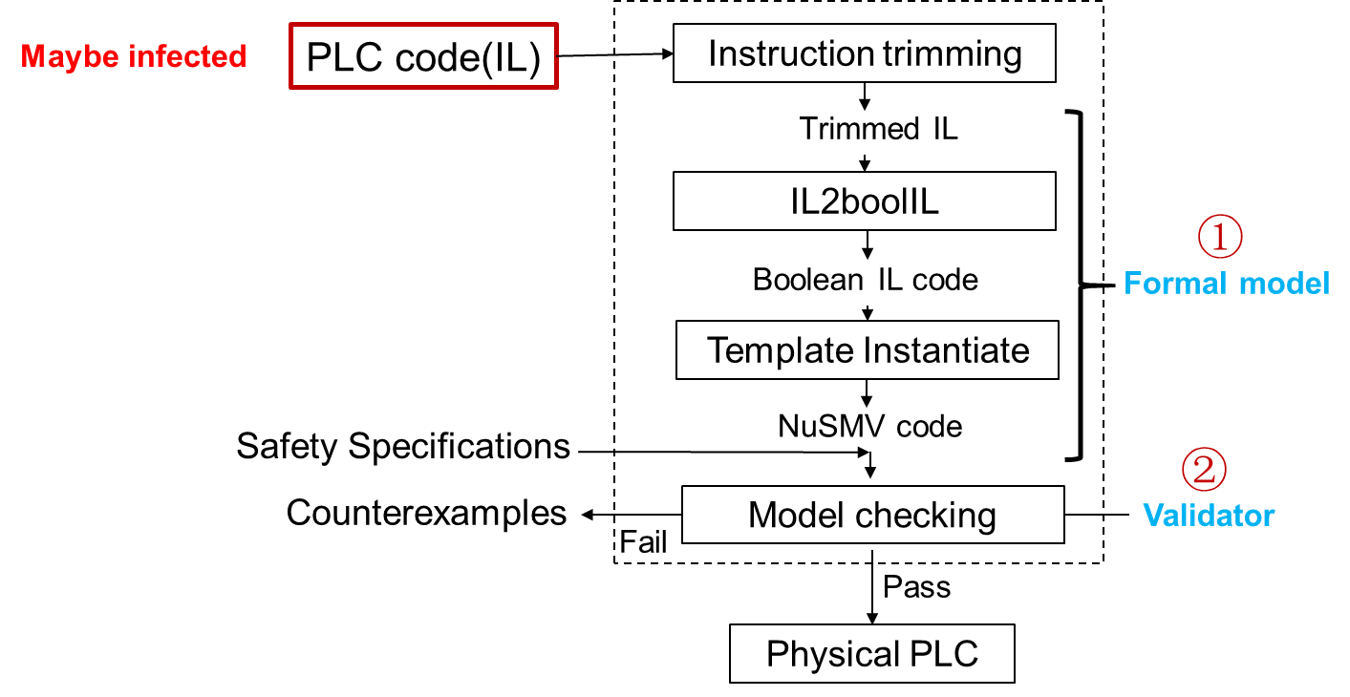
\includegraphics[scale=0.49]{spec/flowchart_spec.png}
\caption{基于规范的入侵检测流程图}
\label{fig21}
\end{figure}

\section{系统建模和入侵检测设计}
\label{sec:matheq}

\subsection{PLC指令表程序介绍}

指令表程序(Instruction  List,IL)是一种较老的PLC编程语言,它使用类似于计算机的一些助记符记号来表示PLC的操作功能,并根据相应的词法和语法写入每一行程序,以实现工业要求的控制目标和运算处理。

指令表程序具有以下特点:

\begin{itemize}
	\item 每条指令包含明确的功能而且变量之间的逻辑关系清晰。 
	\item 类似于汇编语言,与其他四种编程语言相比更适合现有的程序验证方法。 
	\item 系统执行效率高。
	\item 和其他四种编程语言可以直接对应。
\end{itemize}

因此,为了真正了解PLC程序变量之间的逻辑关系,实现PLC程序的形式验证,首先我们必须掌握指令表程序,这也是指令表程序成为我们研究对象的重要原因。虽然国际电工委员会在IEC61131-3中定义了国际标准的指令表程序,但为了提高系统效率的实际应用,以西门子,洛克威尔和三菱PLC为代表的厂商都发展自己的具体指令表程序规范。尽管每个公司对于指令表程序具有不同的命名约定,但是这些指令表程序在逻辑级上的含义是相同的。由于我们更多关注指令表语义的逻辑,PLC厂商这个因素不会影响我们的检测研究。本文将以西门子的指令程序语句表(Statement  List,STL)为对象开始相关研究工作。

在西门子S7-200指令系统中,可以分为基本指令和应用指令。 所谓的基本指令,最初是指代替传统继电器控制系统所要求的指令。 随着PLC的功能越来越强大,越来越多的指令被涉及,基本指令的内容也在逐步地扩展。 它包括基本逻辑指令,操作指令,数据处理指令,表函数指令和转换指令。 基本逻辑指令包括基本位操作指令,逻辑堆栈指令,定时器指令,计数器指令和比较指令。 基本逻辑指令构成指令集的基本逻辑运算功能,是所有其他指令应用的基础。 因此,本文选择基本逻辑指令中的公共指令,开始对象的研究工作。表\ref{spec:il}展示了我们涉及到的常用的基本指令。

%\newcommand{\tabincell}[2]{\begin{tabular}{@{}#1@{}}#2\end{tabular}}
\begin{table}[!htp]
\centering
\caption{IL指令表基本指令表}
\label{spec:il}
\begin{tabular}{|p{1cm}<{\centering}|p{3cm}<{\centering}|p{8cm}<{\centering}|}
\hline
指令 & 指令类别 & 指令描述 \\
\hline
\end{tabular}
\begin{tabular}{|p{2cm}|p{3cm}|p{8cm}|}
\hline
LD & 逻辑指令 & 装载指令,用于网络块逻辑运算的开始。 \\
\hline
LDN & 逻辑指令 & 装载反指令,用于网络块逻辑运算的开始。 \\
\hline
A & 逻辑指令 & 与指令,用于单个常开触点的串联连接。 \\
\hline
AN & 逻辑指令 & 与反指令,用于单个常闭触点的串联连接。 \\
\hline
O & 逻辑指令 & 或指令,用于单个常开触点的并联连接。 \\
\hline
ON & 逻辑指令 & 或反指令,用于单个常闭触点的并联连接。 \\
\hline
S/R & 逻辑指令 & 置位和复位指令。 \\
\hline
OLD & 逻辑堆栈指令 & 或块指令,用于串联电路块的并联连接。 \\
\hline
ALD & 逻辑堆栈指令 & 与块指令,用于并联电路块的串联连接。 \\
\hline
LPS & 逻辑堆栈指令 & 逻辑入栈指令,也称为分支电路开始指令。从堆栈角度看,LPS指令的作用是把栈顶值复制后压入堆栈。\\
\hline
LRD & 逻辑堆栈指令 & 逻辑读栈指令,从堆栈角度看,LRD将第二个堆栈值复制到堆栈顶部。堆栈没有被弹出,但堆栈顶部的旧数值会被破坏。
\\
\hline
LPP & 逻辑堆栈指令 & 逻辑出栈指令,也称为分支电路结束指令。从堆栈角度看,LPP将
将堆栈的一个数值弹出堆栈,第二个堆栈数值称为堆栈数值的新顶部。\\
\hline
TON & 逻辑定时器指令 & 接通延时定时器,用于单一时间间隔的定时。 \\
\hline
CTU & 逻辑计数器指令 & 增计数器,首次扫描其值为0,在计数脉冲输入端CU的每个上升沿计数器计数一次直到32767后停止计数,复位输入端有效值为0。 \\
\hline
JMP/LBL & 控制指令 & 跳转指令和标号指令,使主机可根据不同条件进行判断,选择不同的程序段执行程序 \\
\hline

\end{tabular}
\end{table}

\subsection{PLC程序的形式化建模}

\textbf{定义1:} IL程序网络(network)是由3元组迁移函数表示: \[ \mathcal{T_{IL}}=(C,c_0,\rightarrow) \] 其中
\begin{itemize}
	\item $C$ 是IL程序配置集
	\item $ c_0 $ 是IL程序初始配置集
	\item $ \rightarrow $ 是迁移关系
\end{itemize}
这里每一个IL程序配置$c\in C$可以由\[ c=(\sigma,e,E) \] 其中
\begin{itemize}
	\item $\sigma$ 是IL程序变量状态
	\item $ e $ 是IL程序网络中将要执行的变量
	\item $ E $ 是IL程序网络中未执行的变量集
\end{itemize}

因为没有标准的步骤来验证PLC程序,我们形式建模的目的是为了通过生成中间语言来更好地或直接转换为NuSMV输入程序。PLC程序的形式模型分为两个阶段。对于第一步,我们采用指令表(IL)作为我们的主要研究PLC语言程序,并且我们需要在算法1中将IL代码转换为布尔逻辑代码(boolIL),即给出映射算法$\={h}: IL \rightarrow boolIL$使得对于IL程序中的每个将要执行的元素$e$都能映射到boolIL中的表示$a=\={h}(e)$。在网络中执行IL运算符的顺序由下一个映射决定:$2^{IL}\rightarrow IL$根据已经执行的元素集确定接下来执行哪个元素。而在boolIL中这一动作已由程序计数器执行并定义映射$p: boolIL\rightarrow IN$将程序中每一条指令$a$映射到它所在的行数$pc$。相应的我们给出boolIL语言的定义:

\textbf{定义2:} boolIL程序网络(network)是也由3元组迁移函数表示: \[ \mathcal{T}_{boolIL}=(B,b_0,\rightarrow) \] 其中
\begin{itemize}
	\item $B$ 是boolIL程序配置集
	\item $ b_0 $ 是boolIL程序初始配置集
	\item $ \rightarrow $ 是迁移关系
\end{itemize}
这里每一个IL程序配置$b\in B$可以由\[ b=(\sigma,a,pc) \] 其中
\begin{itemize}
	\item $\sigma$ 是boolIL程序变量状态
	\item $ a $ 是boolIL程序网络中将要执行的语句
	\item $ pc $ 是boolIL程序网络中$a$语句所在的程序行号
\end{itemize}

第一步的主要目的是获得二进制函数输出从复杂的IL代码通过逐行解释上下文和语义在程序中。算法\ref{algo:boolil}首先将完整的程序划分为多个程序块,然后将每个程序块划分为多个网络块部分并初始化所有的集合。其次,我们对每个逻辑和控制指令执行符号解释以获得二进制函数结果。最后,当实现所有IL程序时,每个结果将从存储器输出。

\begin{algorithm}[!htb]
\caption{IL2boolIL算法}
\label{algo:boolil}
\begin{algorithmic}[1]
\Require %算法的输入参数:Input  
IL程序;

\Ensure %算法的输出:Output  
boolIL程序;  

\State 将完整程序划分成多个程序块$V'$并将每个程序块划分为多个网络块$F$
\State 初始化并设置$V'= 1,F=\emptyset$;
\For{each $j \in SUM_{所有网络块部分}$}
\Switch{第$j$个网络块部分}
\Case {$OP$部分}
\For{each $i \in SUM_{本网络块的总行数}$}
\Switch{第$i$行程序指令}
\Case {$LD$($LND$)}
\State 设置相应的变量值为初始值(取反)输入并存入内存; break;
\EndCase
\Case {$A$($AN$)}
\State 设置相应的变量值为(取反)输入与($\&$)上前一指令的运算结果并存入内存; break;
\EndCase
\Case {$O$($ON$)}
\State 设置相应的变量值为(取反)输入或($|$)上前一指令的运算结果并存入内存; break;
\EndCase
\Case {$TON/CTU/S/R$}
\State 定时器/计数器/置位/复位指令,需要进行抽象建模处理; break;
\EndCase
\EndSwitch
\EndFor
\EndCase
\Case {$ALD$($OLD$)}
\State 使前两个指令运算结果执行与$\&$(或$|$)操作并将执行结果入栈; break;
\EndCase
\Case {$LPS/LPD/LPP$}
\State 存入/读取/弹出堆栈中前一指令的运算结果; break;
\EndCase
\Case {$JMP/LBL$}
\State 控制指令,需要进行抽象建模处理; break;
\EndCase
\Case {$=$}
\State 输出内存中的最终结果; break;
\EndCase
\Default
\State Return $S_{x_{init}}$
\EndDefault
\EndSwitch
\EndFor
\State Return $S_{x_{init}}$
\end{algorithmic}
\end{algorithm}

从算法\ref{algo:boolil}我们看出有四类指令程序是无法直接进行解释执行的,因此我们需要对这四类指令进行抽象建模。

\begin{enumerate}
	\item $S/R$指令\\
	\begin{center}
	\framebox[250pt][c]{
	\parbox[c]{100pt}{
	\framebox[60pt][c]{IN}\\
	\makebox[60pt][c]{$\downarrow$}\\
	\makebox[60pt][c]{S/R Out}} $\Rightarrow \begin{cases} S: Out=IN\& Out\\R: Out=!(IN|Out)\end{cases}$ }
	\end{center}
	我们发现$S/R$有自锁的特性,即当$S$的输出$Out$为0时,不管其前面的程序集的输入$IN$为何值,其结果总为0,相应的$R$指令也有类似的特性。

	\item 控制指令$JMP$和$LBL$\\
	\begin{center}
	\framebox[350pt][c]{
	\parbox[c]{80pt}{
	\framebox[60pt][c]{X}\\
	\makebox[60pt][c]{$\downarrow$}\\
	\makebox[60pt][c]{JMP n}\\
	\makebox[60pt][c]{$\downarrow$}\\
	\framebox[60pt][c]{$Y_n(y_n)$}\\
	\makebox[60pt][c]{$\downarrow$}\\
	\makebox[60pt][c]{LBL n}\\
	\makebox[60pt][c]{$\downarrow$}} 
	$\Rightarrow$ $ Y_n=(Y_n \& (y_n|!X)) | (y_n\&X)  = \begin{cases} y_n,~~ if~X=1\\Y_n,~~ if X=0\end{cases}$
	}
	\end{center}
	这里的$X$是$JMP$指令的输入,$Y_n$是$LBL$指令的输入,$y_n$是$Y_n$的初始值。抽象建模后的$Y_n$的输出严格遵循控制指令的语义,即当$X=1$时,控制指令激活并跳过$JMP$和$LBL$的程序,$Y_n$的输出即为初始输出值$y_n$;当$X=0$也能得到类似的结论。
	\item 定时器指令TON\\
	如图\ref{fig22}所示,定时器的端口由输入$IN$、输出$Q$和定时时间$PT$组成,右上方的状态转移图描述了定时器执行过程中的三个状态迁移过程。初始状态$NR$输出$Q$为$false$,输入$IN$未激活置为0;当$IN$激活后但未达到时间要求时,迁移到第二状态$R$,此时输出$Q$仍为$false$;如果在未达到定时时间时,输入被置0则又会回到初始状态$NR$,一旦在激活状态且达到定时时间,定时器会到达它的第三状态$TO$,此时输出$Q$为$true$,如果输入又被置0则又会回到初始状态$NR$。这里要特别说明我们并没有模拟具体的时间,对于是否满足时间要求我们只给出$true$和$false$两个状态。为了便于理解,图的下方给出了简单的例子,定时器$T1$的运算结果由输入$In1$和定时时间状态$T1Ton$共同决定。
	\begin{figure}[!htb]
	\centering
	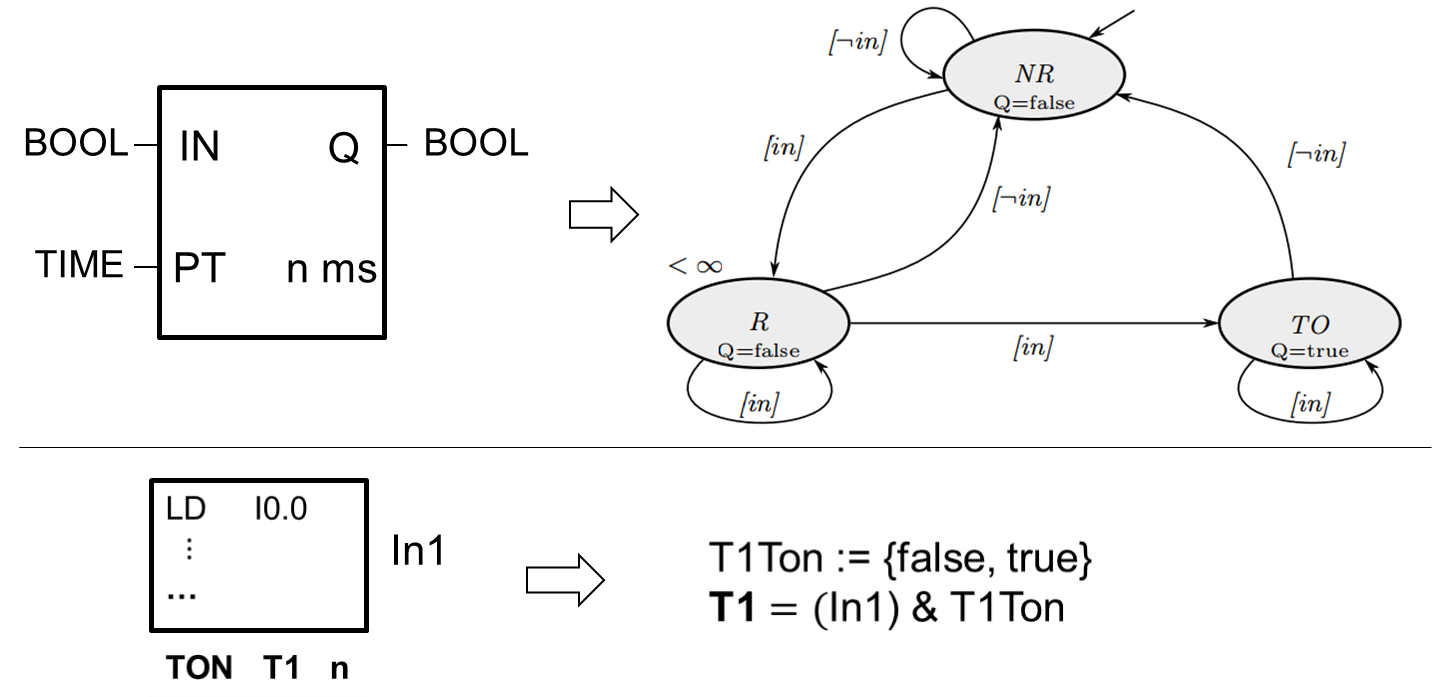
\includegraphics[scale=0.48]{spec/ton.png}
	\caption{TON指令的抽象建模}
	\label{fig22}
	\end{figure}


	\item 计数器指令$CTU$\\
	如图\ref{fig23}左上方所示,计数器的端口由输入$CU$、重置$R$、计数次数$PV$和输出端$Q$(单独的端口)组成,右上方的状态转移图描述了定时器执行过程中的四个状态迁移过程。初始状态输出$Q$为$false$,输入$CU$未激活置为0且重置$R=0$;当$IN$激活后且重置$R=0$但未达到计数次数要求时,迁移到第二种状态即激活状态,此时输出$Q$仍为$false$;如果在未达到计数次数时,输入被置0则又会回到初始状态,一旦在激活状态时未被重置且达到计数次数$N$,计数器会到达它的第三种状态即响应状态,此时输出$Q$为$true$,如果重置$R=0$则会到达第四种状态即重置状态,此时$Q=false$且$PV=0$被重置。为了便于理解,图的下方给出了简单的例子,计数器$C20$的运算结果由输入$C20CU$和计数次数状态$PV$共同决定。

	\begin{figure}[!htb]
	\centering
	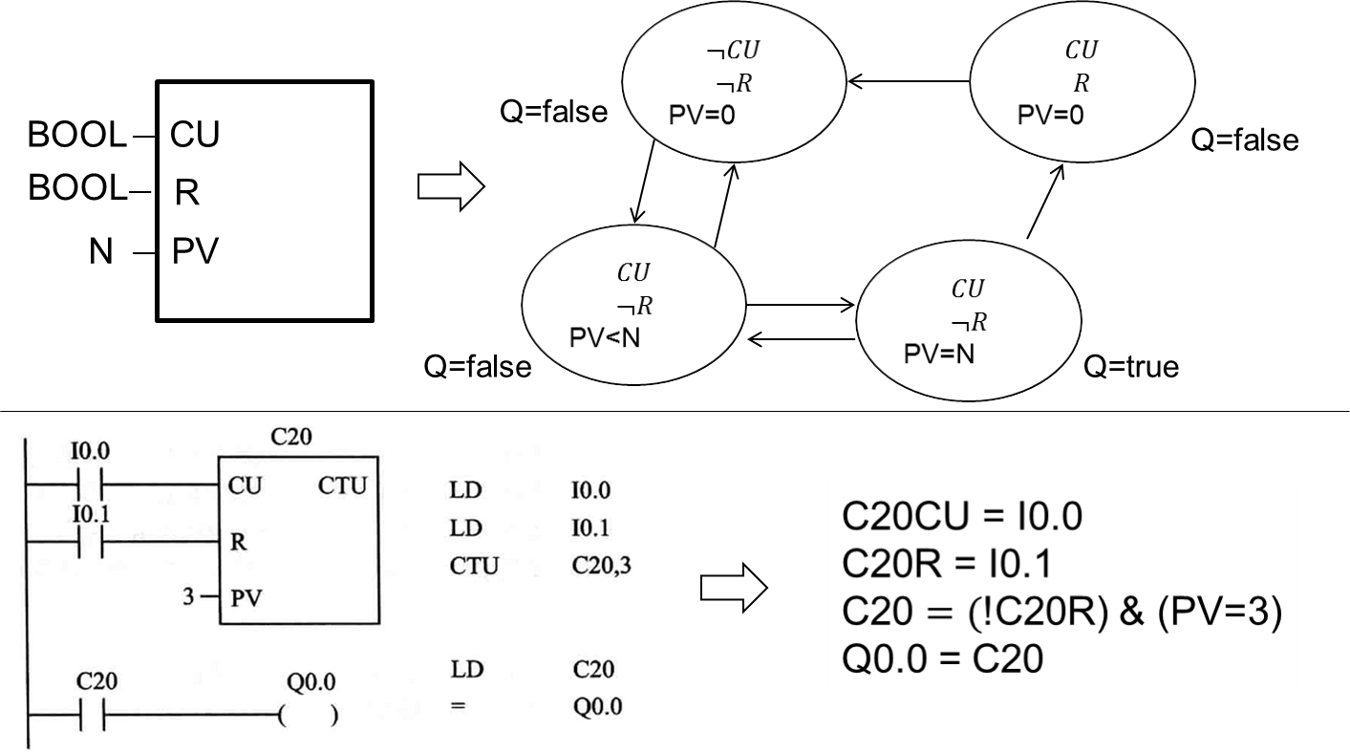
\includegraphics[scale=0.48]{spec/ctu.png}
	\caption{CTU指令的抽象建模}
	\label{fig23}
	\end{figure}
\end{enumerate}

对于步骤二,我们需要通过步骤一的二进制输入函数的输出来实例化验证工具程序模板得到可执行程序模型。在我们的工作中,我们采用NuSMV作为我们的模型验证器。NuSMV是SMV符号模型检查器的重新实现和扩展并用于有限状态系统的形式化验证,它是基于二元决策图(BDD)的第一个模型检查工具。该工具被设计为用于模型检查的开放式架构。 它的目的是可靠地验证工业大小的设计,用作其他验证工具的后端和作为形式验证技术的研究工具。它支持计算树逻辑(CTL)和线性时间逻辑(LTL)中表达的规范的分析,我们可以从我们的控制系统的安全规范中轻松获得。详细的实例化过程如图\ref{fig24}所示。图\ref{fig24}首先实例化所有输入,输出和pc计数。考虑初始化输入和输出是自动生成过程,因此主要任务是在执行下一个输出语句时为每个case语句分配对应pc计数器的执行语句。

\begin{figure}[!htb]
\centering
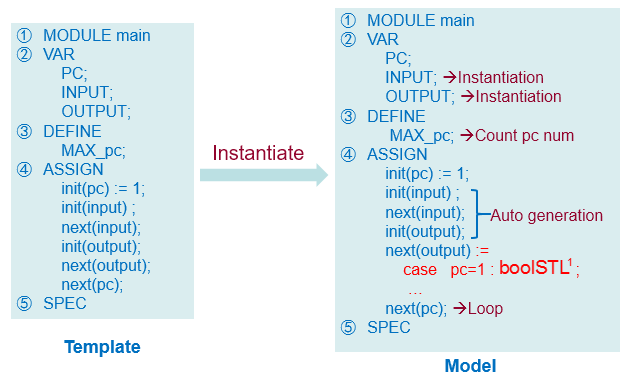
\includegraphics[scale=0.48]{spec/instantiation.png}
\caption{模板实例化过程}
\label{fig24}
\end{figure}

\subsection{模型检测}

由于PLC在每个执行周期使用状态变量来描述状态的变化。因此,我们仅分析单个执行周期来检查所有时间内的安全性规范是远远不够的。在本节中,我们将会给出了完整的模型检测算法来验证PLC程序的形式模型树图是否存在违反安全规范的路径。上一节提出的转换算法是对在所有执行周期里发生的状态变换进行建模并构建形式化模型的执行图,在更详细地阐述模型检测过程之前,我们简要介绍下用于安全规范的CTL。

\subsubsection{计算树逻辑CTL}

\textit {计算树逻辑},或简称CTL,是一个\textit {分支时间}逻辑,意味着它的时间模型是一个树状结构并且未来状态没有确定;在未来有不同的路径,任何一个都可能是实现的路径\parencite {klein2005fault}。

\textbf{定义 3}我们通过Backus Naur形式定义CTL公式:
\begin{equation} 
\begin{split}\phi :: = \bot | \top | p |(\neg\phi) | (\phi\wedge\phi) | (\phi\vee\phi) | (\phi\rightarrow\phi) | AX\phi |\\ EX\phi | AF\phi | EF\phi | AG\phi | EG\phi | A[\phi U \phi] | E[\phi U \phi]\end{split}
\end{equation}
这里\textit{p }是一组原子公式.

注意到每个CTL时间连接是一对符号,第一对是A和E之一。A意思是“沿所有路径”(\textit {不可避免}),E意思是“至少(存在)一个路径”(\textit {可能})。 第二对是X,F,G或U,分别表示“下一个状态”,“某些未来状态”,“所有未来状态(全局)”和“直到某个状态”。 例如,E[\textit{$\varphi{}$}$_{1 }$U \textit{$\varphi{}$}$_{2}$]中的符号对是EU。在CTL中,诸如EU的符号对是不可分割的。注意AU和EU是二进制的。 符号X,F,G和U不能出现在A或E之前;类似地,每个A或E必须具有X,F,G和U中的一个。

\subsubsection{规范检测}

我们定义的过程安全规范是安全描述和控制系统与物理设备的约束行为。 基于规范的入侵检测尝试从控制逻辑模型$M$验证所有安全规范。如果发现反例,则给出警报可能存在恶意攻击注入智能控制器程序。

规范是由\textit {specifications}的有序列表组成且名称为\textit {id}的规范具有以下语法:
\[\begin{split}
id:  <input [input-list]> <output [output-list]> \\
<INIT [init-input-list]> <UNIQUE> \varphi
\end{split}
\]

例如,我们可以给出设备按钮的简单描述:“按下启动按钮时,原料M的阀门打开”,对应的规范如下面的\textit {lbutton}所示:
\[\raggedright
{ \textit{lbutton }: input~ \textit{launch}}{\small {^\ast} }{\large
~output~ \textit{v}_{M} ~INIT~ \textit{launch}}{\small {^\ast} }
\]

\[\raggedright
\textit{launch}^{*}\Rightarrow AX \textit{v}_{M}
\]

安全属性\textit {$ \varphi {} $}在计算树逻辑(CTL)中的定义是规范的唯一强制性的部分。CTL的规范定义的$ input $和$ output $来自控制程序的形式化模型集$ IO_\phi $,即$ \{input-list\} \cup{}  \{output-list\}$
$\subseteq{}$ \textit{$IO_\phi$}。验证过程分为三个步骤:基于规范的入侵检测将会通过控制逻辑模型$ M $验证\textit{$\phi{}$ }中的所有安全规范。
\begin{enumerate}
	\item 选择 $\phi$:~$\phi \leftarrow Pop(SPECs)$ .
	\item 将形式化模型和物理设备变量的输入$input$和输出$output$映射集$IO_{M}$ 应用到$\phi$中. 定义为$\phi/IO_M$,即“在映射集$IO_M$下得到的属性$\phi$”.
	\item 验证 $M \vert{}$= \textit{$\phi/IO_M$}.
\end{enumerate}

这三个步骤适用于给定控制逻辑模型的所有安全规范,如算法\ref{algo:modelcheck}所示。首先,我们需要初始化输入和输出映射集$ IO_M $和控制逻辑模型$ M $,然后我们需要遍历安全规范$ SPECs $中的每个属性,并转换为$ IO_M $映射下的模型符号CTL规范。之后将通过MuSMV验证工具处理每个模型符号CTL规范$M \vert{}$= \textit{$\phi/IO_M$}。 如果存在不能通过模型检查并生成反例的任何属性,那么基于规范的入侵检测将激活警报机制,需要工作人员检查可能存在的某些注入当前系统程序的恶意代码。

\begin{algorithm}[h]
\caption{模型检测}
\label{algo:modelcheck}
\begin{algorithmic}[1]
\Require %算法的输入参数:Input  
安全 $SPECs$, 输入和输出映射集 $IO_M$和控制逻辑模型$M$ 

\Ensure %算法的输出:Output  
如果检测到存在攻击,则返回 $\mu_{CE}$并激活报警机制;否则返回安全通过; 
\State 初始化$IO_M$ 和 $M$
\For{each $\phi \in SPECs$}
\State $\phi \leftarrow IO_M$
\If { NOT $M \vert{}$= \textit{$\phi/IO_M$}}
\State $\mu_0 \leftarrow \textit{Counterexample Path}$
\State $\mu_{CE} \leftarrow \mu_{CE}\cup \mu_0$
\EndIf
\EndFor
\If {$\mu_{CE}.size() > 0$}
\State \textbf{激活} $alarm$
\EndIf
\State \textbf{return} $\mu_{CE}$

\end{algorithmic}
\end{algorithm}	

\section{实验仿真}
\label{sec:insertimage}

为了证明所提出的基于规范的检测方法的可行性和性能,我们给出了基于自动重合闸控制系统的仿真实验。该系统的功能是在瞬时故障发生时使用重合闸恢复电源,并在发生永久故障时使用备用电源。 该系统有9个输入(来自系统的测量)和11个输出(从PLC到执行器的信号)。 图\ref {fig29}显示了主电气连接图,图\ref {fig210}显示了系统的输入和输出映射表。

\begin{figure}[!htb]
\centering
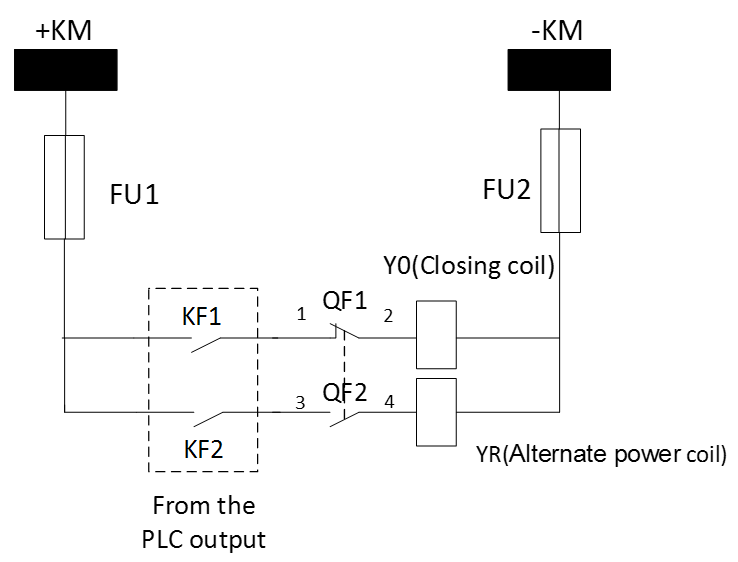
\includegraphics[scale=0.48]{spec/diagram.png}
\caption{自动重合闸控制系统主电气连接图}
\label{fig29}
\end{figure}

\begin{figure}[!htb]
\centering
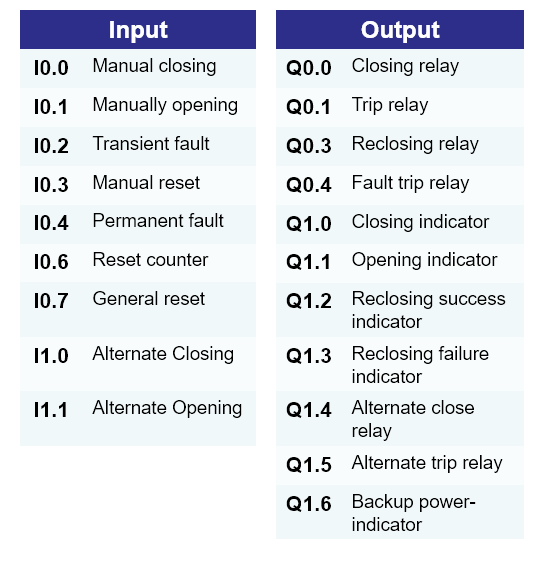
\includegraphics[scale=0.45]{spec/mappingTables.png}
\caption{自动重合闸控制系统的输入和输出映射表}
\label{fig210}
\end{figure}

Firstly, we build the formal model of control system, Fig.~\ref{fig211} shows how we transfer the part of instruction lists to boolean logic program and get binary function output from the complex IL code using algorithm 1. Fig.~\ref{fig12} presents part of instantiated performable code model for NuSMV tool, and the model should be written to the file ending with '.smv'.
首先,我们构建控制系统的形式模型,图\ref {fig11}显示了如何使用算法\ref{algo:boolil}将部分指令表程序去重处理并获得二进制函数输出进而转化为布尔逻辑指令表boolIL程序。图\ref {fig212}提供了NuSMV工具的实例化可执行代码模型的一部分,并且该模型应该写入以“.smv”结尾的文件。
\begin{figure}[!htb]{}
\centering
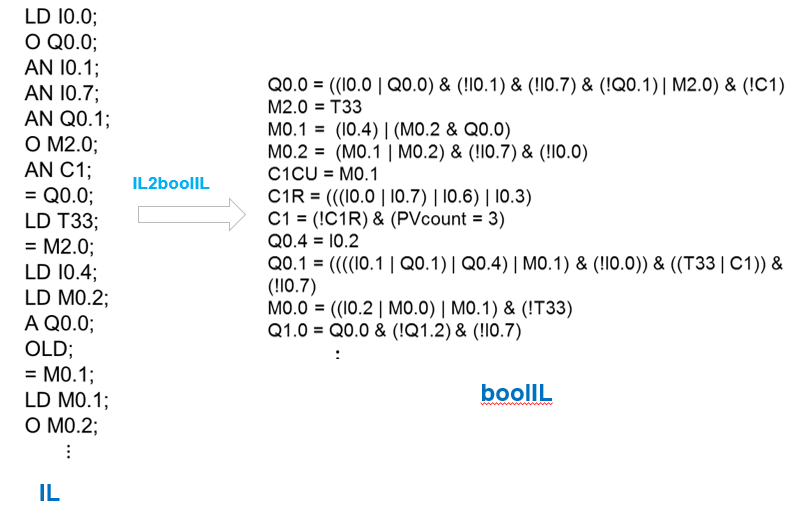
\includegraphics[scale=0.49]{IL2boolIL.png}
\caption{IL2boolIL转化过程}
\label{fig211}
\end{figure}

\begin{figure}[!htb]
\centering
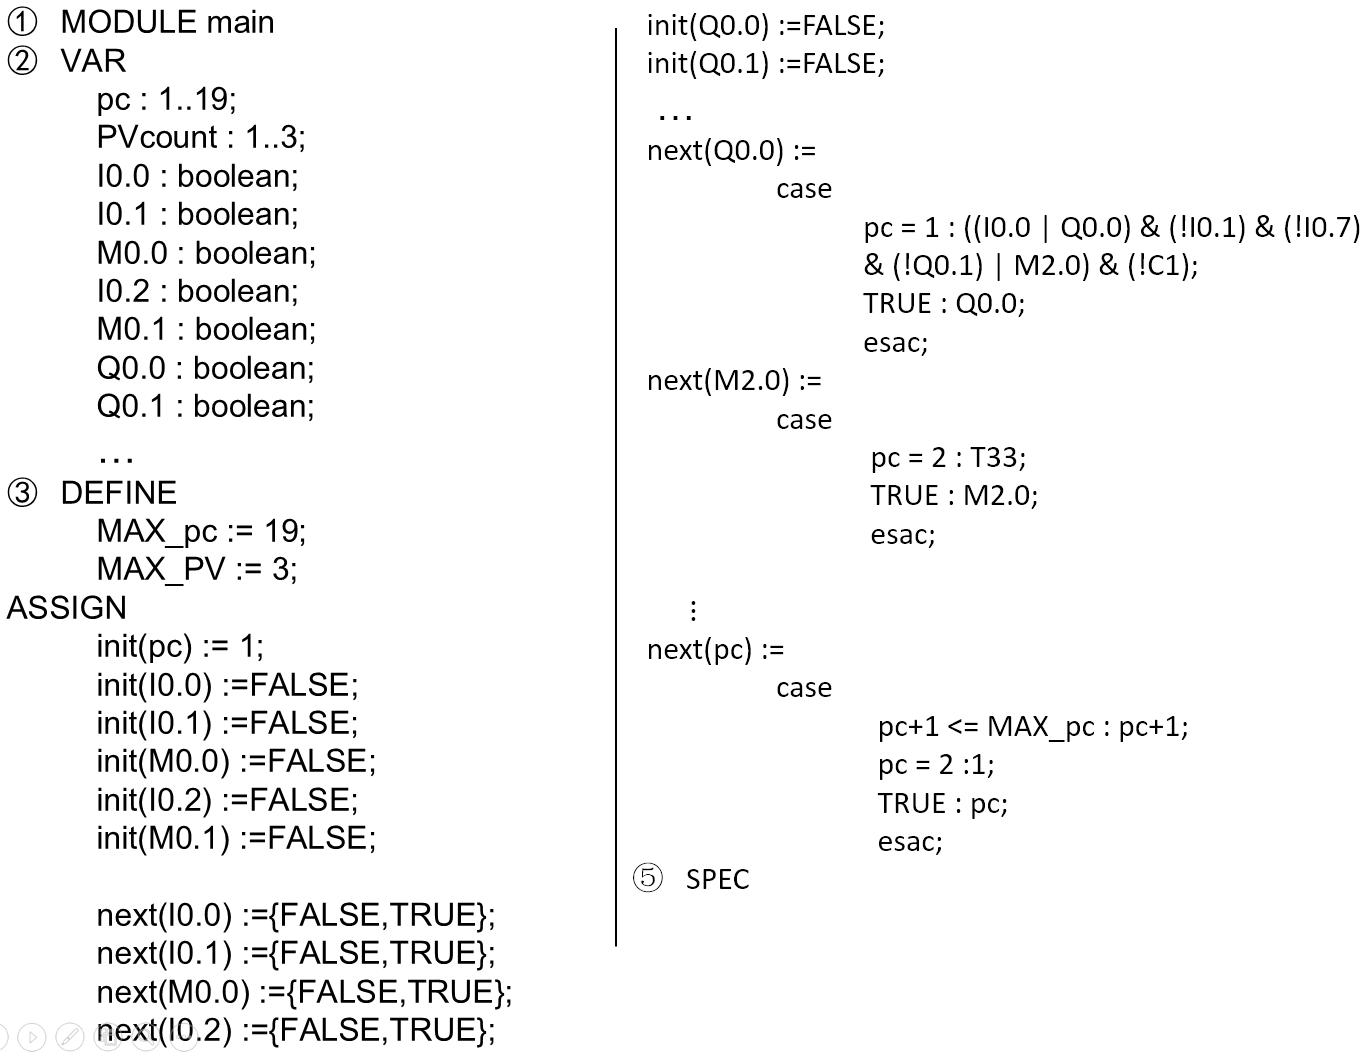
\includegraphics[scale=0.47]{Instantiate.png}
\caption{实例化过程}
\label{fig212}
\end{figure}
To make sure automatic reclosing control system work in expected status, we design 7 main requirements as follows:
为了使自动重合闸系统工作在预期的状态,我们为系统设计了7条主要的安全规范:
\begin{itemize}
	\item 关闭指示器在手动关闭回路时工作正常。
	\item 手动打开回路时,跳闸指示灯工作正常。
	\item 当模拟瞬态故障时,自动重合闸继电器工作且重合闸成功指示灯闪烁。
	\item 模拟永久故障时,自动重合闸继电器不工作且重合闸故障指示灯闪烁。
	\item 当模拟永久故障时,需要自动交流电源为用户提供电源,并且正在使用的备用电源指示灯可以顺利工作。
	\item 它可以手动关闭备用回路。
	\item 它可以手动打开交替回路。
\end{itemize}

After we obtain the program model of the automatic reclosing control system, we require to construct specification of CTL form. For instance, from the first requirement we can draw the CTL specification as follow:\[\begin{split}
\bullet &AG(I\_ManualClosing\&(! I\_ManualOpening) )\&(! I\_GenReset) \\&-> AF(O\_ ClosingRelay));\\\bullet &AG((O\_ ClosingRelay \& (! I\_GenReset)) \\&-> AF(O\_ClosingIndicator));
\end{split}
\]

However, the valuables in them all are physical, the inputs and outputs mapping tables can help to solve it. The specifications of CTL will be redefined over names given after \textit{input} and \textit{output} keywords from the mapping. The final CTL specifications are as follows:
\[\begin{split}
\bullet &AG(I0.0\&(! I0.1) )\&(! I0.7) -> AF(O0.0));\\\bullet &AG((O0.0 \& (! I0.7)) -> AF(O1.0));
\end{split}
\]
Similarly, the rest requirements all can be converted to CTL specifications.

If there is no any attack on control program, after verifying all the safe specifications, each specification will present 'T' standing for currently being the security state. The results of detection are show on Table 1.

\begin{table}[!htb]
\centering
\begin{tabular}{cccccccc}

\hline
Cycle & 1 & 2 & 3 & 4 & 5 & 6 & 7\\

1 & T & T & T & T & T & T & T\\

2 & T & T & T & T & T & T & T\\

3 & T & T & T & T & T & T & T\\

4 & T & T & T & T & T & T & T\\

~$\colon$ & ~$\colon$ & ~$\colon$ & ~$\colon$ & ~$\colon$ & ~$\colon$ & ~$\colon$ & ~$\colon$\\
\hline
\end{tabular}
\caption{Verifying result without attack}
\end{table} 

If there exists any attack on control program, after verifying all the safe specifications, several continuing specifications will present 'F' meaning that currently the unsafe state is happening. The results of detection are show on Table 2. Once facing this situation, the related attacked part of device will shutdown instantly and alert alarm. Then engineers require to check the third and sixth specification to repair the control system.

\begin{table}[!htb]
\centering
\begin{tabular}{cccccccc}

\hline
Cycle & 1 & 2 & 3 & 4 & 5 & 6 & 7\\

~$\colon$ & ~$\colon$ & ~$\colon$ & ~$\colon$ & ~$\colon$ & ~$\colon$ & ~$\colon$ & ~$\colon$\\

112 & T & T & F & T & T & F & T\\

113 & T & T & F & T & T & F & T\\

114 & T & T & F & T & T & F & T\\

~$\colon$ & ~$\colon$ & ~$\colon$ & ~$\colon$ & ~$\colon$ & ~$\colon$ & ~$\colon$ & ~$\colon$\\
\hline
\end{tabular}
\caption{Verifying result with attack}
\end{table} 

\section{本章小结}
\label{sec:insertimage}


%# -*- coding: utf-8-unix -*-
%%==================================================
%% chapter02.tex for SJTU Master Thesis
%% based on CASthesis
%% modified by wei.jianwen@gmail.com
%% Encoding: UTF-8
%%==================================================

\chapter{基于异常数据的入侵检测设计}
\label{chap:data detection}

\section{引言}
\label{sec:intro}

在上一章节中,我们讨论了过程控制系统在远程输入信号采集和传输过程中遭受的数据注入攻击并阐述如何构造较为隐蔽的错误序列注入攻击。事实上大多数控制应用(例如监控和数据采集(SCADA))都需要保证严格的安全性,因为一旦由任何异常故障或恶意攻击引起的错误甚至恶意行为都会导致物理设备甚至整个系统遭受无法逆转的破害。在本章节中,我们主要针对控制系统中控制器接收来自本地和远程输入信号的完整性和安全性设计了基于异常数据的入侵检测机制,并且我们考虑到错误序列注入攻击序列构造特性设计了有效的FSI检测算法。

\section{入侵检测方案概述}
\label{sec:list}

考虑到前一章节中描述的威胁模型,来自远程终端单元(RTU)或PLC的远程传感器的信号数据也面临数据集成攻击,我们将入侵检测机制放在PLC或者RTU可编程控制器与物理设备连接的输入和输出两端。从传感器测量的每个数据或信号都需要经过监测并验证完整性,一旦存在未能通过检测的观测数据机制立即给出报警并定位可能受攻击的传感器位置。具体实现时,与构造攻击采用的模型辨识类似,首先收集PLC控制器与系统物理设备之间传输的信号和内存数据形成输入和输出向量采样数据库,我们辨识出能够高度复现待检测系统的无故障离散事件模型。然后针对异常数据注入攻击的特点,分为两个阶段设计异常数据检测算法。第一阶段将监测的控制器输入信号与模型的预期输出残差对比判断是否数据异常;第二阶段对隐蔽的错误序列注入攻击设计额外FSI检测算法来避免此类型的攻击。最后对检测存在异常的数据分析判断,定位到具体攻击源并给出相应的应对措施。



\section{系统建模和入侵检测设计}
\label{sec:matheq}

\subsection {攻击类型}

对于异常数据注入攻击,主要存在两种类型。一类是\textit {蛮力和类故障攻击},例如由Mclaughlin等人提出的拥有控制意识的FDI攻击\parencite{mclaughlinS2014}和由Pang等人设计的伪装假数据攻击\parencite{pang2015}。 然而这类攻击是实现具体的任务和目标是销毁受控系统,但是没有考虑受感染系统本身的安全机制,所以很容易被成熟的故障检测机制检测到\parencite{roth2012,garcia2012}。另一类是\textit {隐蔽和避免故障检测的攻击},这类攻击的典型代表就是我们前一章节构造的错误序列注入攻击。这种类型的攻击要求攻击者熟悉的受感染系统的物理变量与控制器连接配置信息并能够访问传感器,因此它可以避开系统故障检测。

\subsection {检测方法}

我们在图\ref {fig28}中创建了一个两阶段检测的流程示意图,用于描述基于前一节提到的两种类型的攻击进行基于异常数据的检测过程。 一方面图\ref {fig28}显示了结合观测到的I$I/O$向量数据库和辨识的离散事件模型,我们首先对a)类攻击\textit {蛮力和类故障攻击}进行残差对比检测。另一方面我们需要验证当前观测的向量值映射到模型中的状态的前一状态是否存在多个后继状态,对应到状态转移图即当前对应的状态只是上一状态的某个分支其,如果是的话我们针对b)类攻击\textit {隐蔽和避免故障检测的攻击}进行特定的FSI检测。最后在经过两个阶段检测之后,我们将检测结果进行分析并定位以获得攻击源的具体位置。

\begin{figure}[!htb]
		\centering
		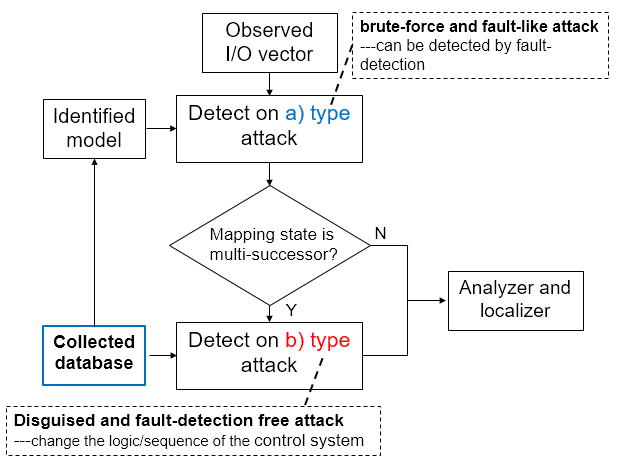
\includegraphics[scale=0.35]{dataD/flow-chart.png}
		\caption{基于异常数据检测的流程示意图}
		\label{fig28}
	\end{figure}

考虑到我们的主要检测目标是能够改变控制系统的逻辑或进程的错误序列注入攻击,由于FSI攻击来自辨识的模型的相同输出确保其不会被故障机制直接检测,而且通过选择具有恶意执行逻辑的适当长度的错误序列注入到控制器的输入信号中来破坏系统。算法\ref{algo:abd}显示了基于异常数据的检测过程。第一步是通过类似构造攻击模型辨识过程来获得待检测系统NDAAO模型,然后根据残差计算每个当前观测的$I/O$向量值与模型的预期输出是否一致。如果不一致则认为在当前模型的状态估计集为空即不存在任何可行的下个状态,此时很可能遭受\textit{蛮力和类故障攻击},否则我们需要检查先前状态估计集模$|\hat{X}_{t-1}|$的大小是否大于1,如果是的话可能存在错误序列注入攻击并进行第二阶段FSI攻击的检测。

由上章节中FSI序列的定义式(2-7)中长度为$n$的序列$s$满足的必要条件是$s\notin L_{Obs}^n$,所以我们需要增加记录每一观测向量值并判断从观测周期初始向量到当前观测向量组成的观测序列$\phi$是否存在于原始用来辨识模型的采样序列库中,如果不存在的话则可以判断系统受到FSI攻击。为了使检测更加有效,我们只保留每次检测时序列满足$ \varphi$属于$\gamma'$任意子字符串的$\gamma'$并将$\gamma'$保存于$\varSigma'$,主要目的是删除没有用到的验证序列集并保留有效的序列以验证观测序列$\phi$是否属于采样序列库的子串。 此外介于相邻两个多后继状态之间的序列是唯一的,我们仅仅判断$ \varphi $和$ \gamma $的多后继映射向量(包括当前向量)序列更快地进行验证。 最后判断当前估计状态集$|\hat{X}_{t}|$是否是否等于1,如果不是的话我们把控制系统视为受到\textit {隐蔽和避免故障检测的攻击},否则控制系统将安全地通过检测即没有受到任何攻击。

\begin{algorithm}[h]
		\caption{基于异常数据的检测算法}
		\label{algo:abd}
		\begin{algorithmic}[1]
			\Require %算法的输入参数:Input  
			辨识的NDAAO模型, 新观测的$I/O$向量$\varphi(t)$, 模型的状态估计$|\hat{X}_{t-1}|$, 和用于模型辨识的采样序列库$\varSigma$ \\  
			\Ensure %算法的输出:Output  
			是否通过检测,如果没有的话系统可能受到的攻击类型并给出系统受攻击的路径和传感器位置$locatePair$。 \\
			\If {$|$\^{X}$_{t-1}$$| > 0$}
			\State \^{X}$_{t}$ $\leftarrow \{x\in X|\exists x_{pre}\in$ \^{X}$_{t-1}$$:x\in f(x_{pre}) \wedge IO(\lambda(x_{pre}),\lambda(x))=IO(\lambda(x_{pre}),\varphi(t))\}$
			\If {$|\hat{X}_t|=0$}
			\State $locatePair\leftarrow locatePair((\varphi_{init},...,\varphi(t)),IO(\lambda(x_{pre})\cup IO(\lambda(x_{pre}),\varphi(t)))$
			\State \textbf{return} \textit{蛮力和类故障攻击}
			\EndIf
			\If {$deg(\hat{X}_{t-1})>1$}
			\State $\phi \leftarrow (\varphi_{init},...,\varphi(t))$
			\For {each $\gamma \in \varSigma$}
			\State 保留满足 $\varphi 属于\gamma'$子串的$\gamma'$ 并且 $\varSigma' \leftarrow \gamma'$
			\State $\phi_{ms} \leftarrow$ 保留对应到模型中的多后继向量(包括当前向量)的 $\phi$的序列
			\State $\gamma_{ms} \leftarrow$ 保留对应到模型中的多后继向量(包括当前向量)的 $\gamma$的序列
			\State $\phi\leftarrow \phi_{ms}, \gamma\leftarrow \gamma_{ms}$
			\If {$\phi \notin substring(\gamma)$}
			\State $\hat{X}_t \leftarrow \emptyset$
			\State break
			\EndIf
			\EndFor
			$\varSigma \leftarrow \varSigma'$
			\EndIf
			\Else
			\State $\hat{X}_t \leftarrow \{x\in X|\lambda(x)=\varphi(t)\}$
			\EndIf
			$\hat{X}_{t-1}\leftarrow \hat{X}_t$
			\If {$|\hat{X}_t|=1$}
			\State \textbf{return} \textit{安全通过检测}
			\Else
			\State $locatePair\leftarrow locatePair(\phi,IO(\lambda(x_{pre})\cup
			IO(\lambda(x_{pre}),\varphi(t)))$
			\State \textbf{return} \textit{隐蔽和避免故障检测的攻击}
			\EndIf
		\end{algorithmic}
	\end{algorithm}

对于攻击定位,一旦存在任何攻击我们需要分析并存储相关的受攻击路径和传感器。 值得注意的是,我们可以通过比较采样的序列库和保存的受攻击路径(序列)来定位具体哪个部分受到攻击。 为了实现更好的定位精度,我们还需要保存表示当前观测向量和前一个向量之间的驱动事件向量分量,例如温控设备开关和温度信号等物理变量。此外相应的采样序列的驱动事件变量分量应该被记录以定位所有可能的感染的传感器。

\section{实验仿真}
\label{sec:insertimage}

To prove the performance of the proposed method for anomaly-based Detection, another case study is presented. The simulated system is a temperature control system whose function is to satisfy requirement of the temperature and allocate the busy time peak power to the non-busy time with 5 subsystems. The system has 10 inputs (measurements from the system) and 5 outputs (signals from PLC to the actuators). Fig.~\ref{fig13} shows the brief structure of the temperature control system. Fig.~\ref{fig14} presents the simulink layout of the temperature control system.
为了证明所提出的基于异常数据的检测方法的性能,我们给出了基于Dspace实时仿真平台的攻击检测验证实验。DSPACE实时仿真系统由德国dSPACE公司开发,基于MATLAB/Simulink控制系统开发及硬件和软件仿真硬件和软件工作平台,与MATLAB/Simulink/RTW完全无缝连接。DSPACE实时系统具有强大的实时性,高可靠性,良好的可扩展性等特点。DSPACE硬件系统具有高速计算能力,并配有丰富的I/O支持,用户可根据需要进行组合;软件环境,功能强大且易于使用,包括自动代码生成/下载和测试/调试的工具集。DSPACE硬件和软件现在已成为快速原型设计和实时平台的硬件在环仿真的首选。图\ref{fig112}展示了Dspace图片且Dspace详细的技术规则如表\ref{algo:dspace}所示。

	\begin{figure}[!htb]
		\centering
		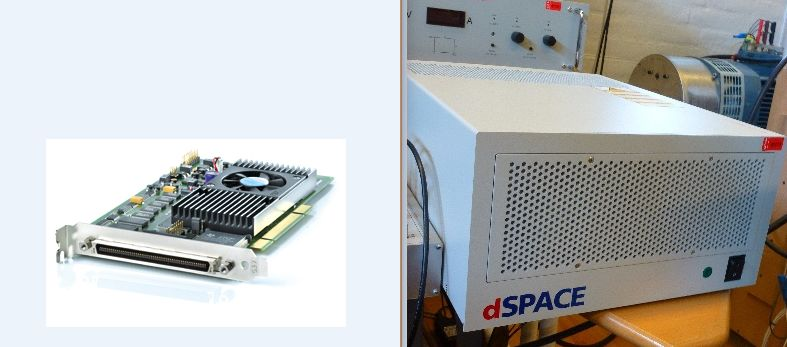
\includegraphics[scale=0.26]{dataD/dspace.jpg}
		\caption{Dspace图片}
		\label{fig112}
	\end{figure}

\begin{table}[!htb]
\caption {ds1006的技术规则}
\label{algo:dspace}
\begin{tabular} {|p{4cm}|p{10cm}|} \hline \hline
  参数&规格\\ \hline
  处理器&四核AMD皓龙处理器2.8 GHz,4 x 64 kB L1数据高速缓存,4 x 64 kB L1指令高速缓存,4 x 512 kB L2高速缓存,6 MB L3高速缓存\\ \hline
  定时器&每个内核:3个通用定时器,多处理器系统的同步时基单元(STBU)\\ \hline
  中断控制器&每个内核:一个中断控制器,具有18个不同的中断源,连接的I/O板的中断源可以通过内部Gigalink从每个内核处理。 \\ \hline

  接口&RS232接口,标准UART允许传输速率高达115.2 Kbaud(串行)\\ \hline
  接口(连接到I/O板)&PHS ++总线接口,用于模块化I/O配置的32位I/O总线(第374页),峰值传输速率为20 MB / s,新I/O板,最多64个PHS总线中断。 \\ \hline

  主机接口&一个全尺寸16位ISA插槽,通过8个16位I/O端口(ISA总线)接口\\ \hline

  多处理器系统&构建具有更多DS1006处理器板的多处理器系统,多达20个DS1006处理器板,每个DS1006上通过一个DS911千兆模块最多4条高速链路,可能的电缆长度可达100米\\ \hline

  物理特性&340 x 125 x 15毫米(13.4 x 4.9 x 0.6英寸)(物理尺寸)\\ \hline
  物理特性&0-40°C(32-104°F)(环境温度)\\ \hline
  物理特性&主动冷却(风扇)(冷却)\\ \hline
  物理特性&(电源)ISA总线:+5 V±5%2.0 A(无DS911),+5 V±5%3.0 A(DS911至模块版本2.0),+12 V±5%连接器:+5 V±5%20 A. \\ \hline
  内存&1 GB DDR2-800 SDRAM本地内存,用于应用程序和动态应用程序数据,4 x 128 MB DDR2-267 SDRAM全局内存,用于主机数据交换\\ \hline\hline
\end{tabular}
\end{table}

仿真的系统是一个温度控制系统,其功能是满足温度要求,并将繁忙时间峰值功率分配给5个子系统的非繁忙时间。 系统有10个输入(来自系统的测量值)和5个输出(来自控制器到执行器的信号)。图\ref{fig113}显示了温度控制系统的简要结构。图\ref {fig114}介绍了温度控制系统的结构示意图。
	
	\begin{figure}[!htb]
		\centering
		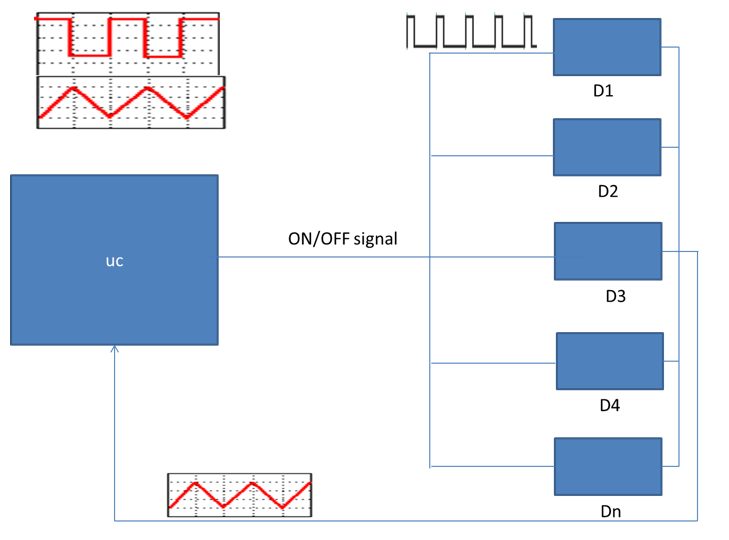
\includegraphics[scale=0.26]{dataD/Temperature.png}
		\caption{Temperature control system}
		\label{fig113}
	\end{figure}
	
	\begin{figure}[!htb]
		\centering
		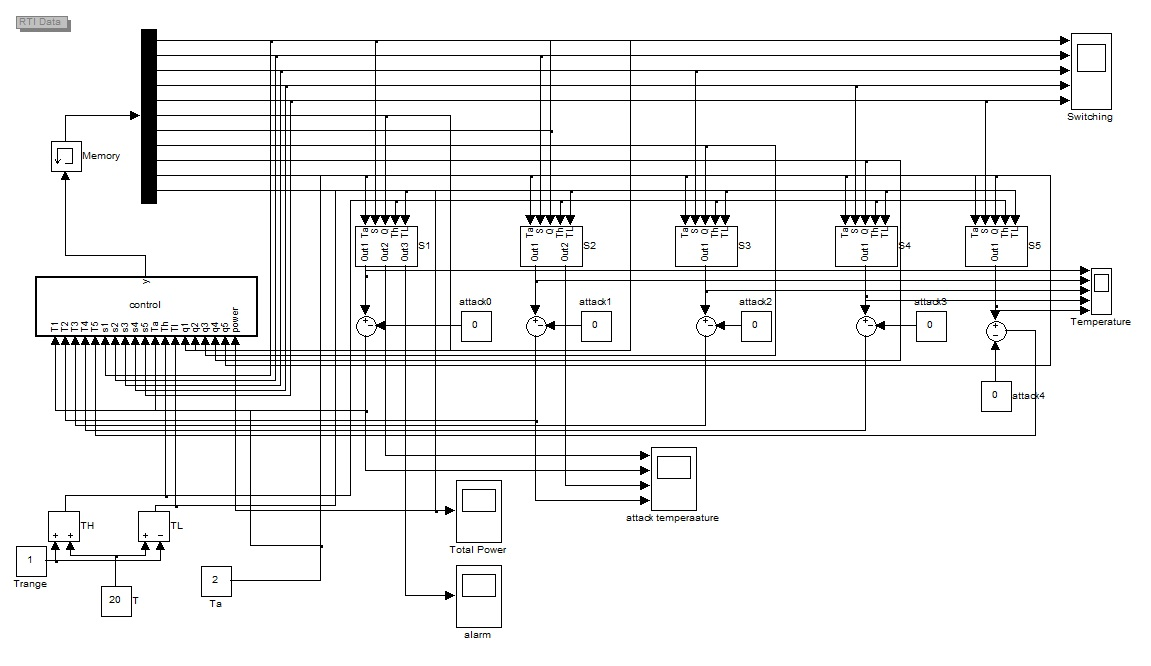
\includegraphics[scale=0.34]{dataD/simulink_attack.jpg}
		\caption{simulink layout of the system}
		\label{fig114}
	\end{figure}
	
	Firstly, we implement \textit{brute-force \& fault-like attack}. We just make random data injection or sequence on the temperature sensors of the system. We execute two kinds of detection:fault-detection and anomaly-based detection. From the result, we obtain that both detection can work perfect. Fig.~\ref{fig15} and Fig.~\ref{fig16} show the detection result of the attack.
	首先,我们对控制系统实行蛮力和类故障攻击,在系统控制器的输入端和温度传感器采集信号端之间我们注入随机的数据或者数据序列。然后我们对其进行两种不同的检测机制:故障检测和基于异常数据的入侵检测机制。从最后的检测结果来看,两种检测都能很好的完成攻击的检测和报警,图\ref{fig115}和图\ref{fig116}分别展示了检测结果。
	
	\begin{figure}[!htb]
		\centering
		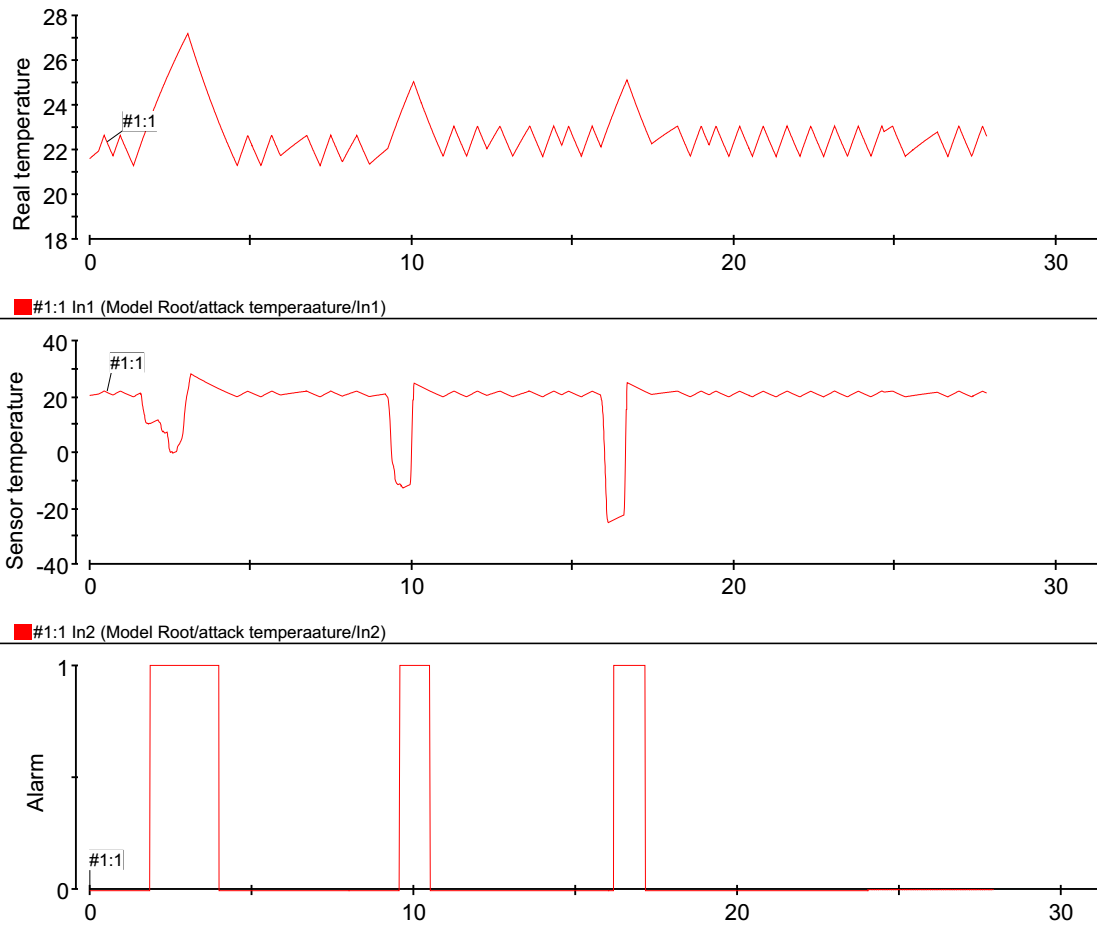
\includegraphics[scale=0.26]{dataD/normalFaultDetection.png}
		\caption{用故障检测机制检测蛮力和类故障攻击}
		\label{fig115}
	\end{figure}
	
	\begin{figure}[!htb]
		\centering
		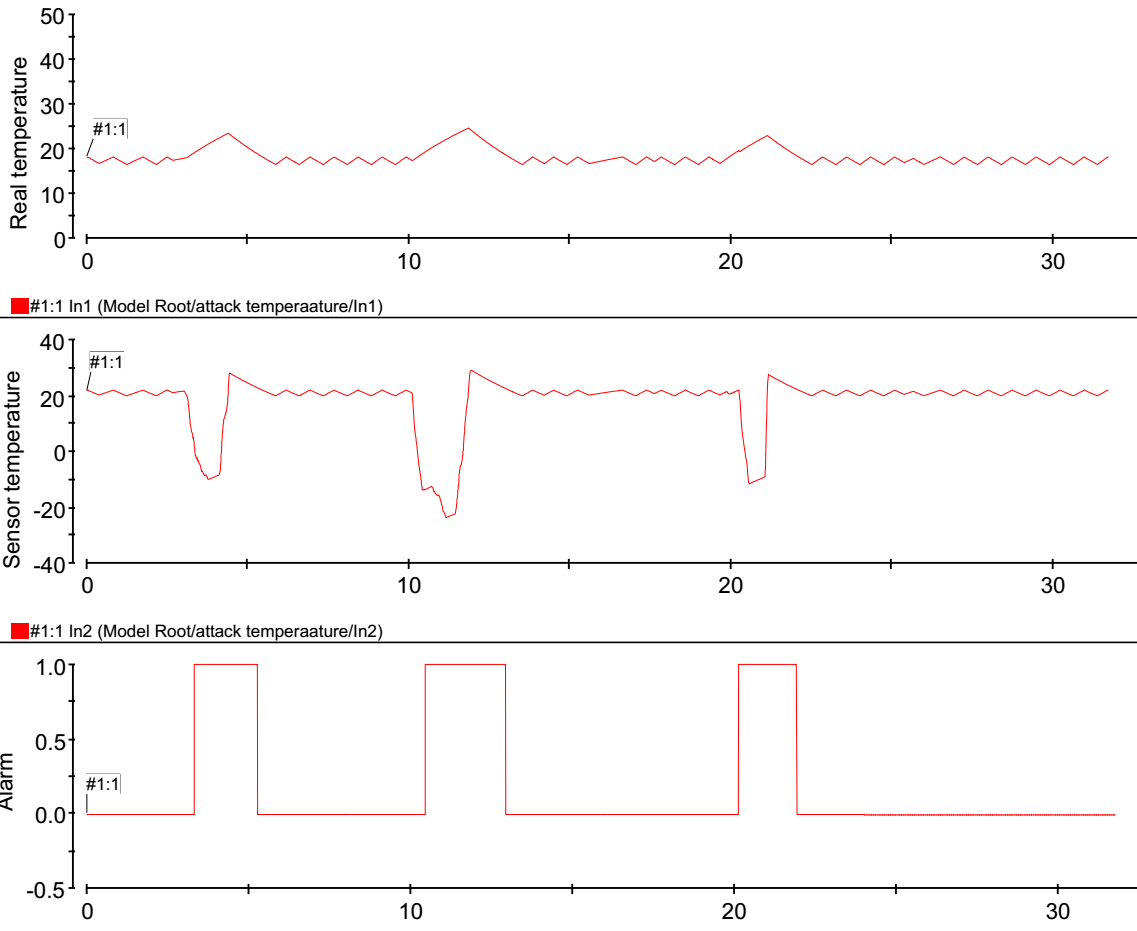
\includegraphics[scale=0.26]{dataD/normalAnomalyDetection.png}
		\caption{用基于异常数据的入侵检测机制检测蛮力和类故障攻击}
		\label{fig116}
	\end{figure}
	
	For the first type of attack, two detection both do the same algorithm to check new observed signal vector according to the expected output. Once any attack is detected, we will take care those comprised sensors, in 
	Fig.~\ref{fig17} those are $Ta3,s3,s4$ and $Tb1,s1,,s2,s3,s4,s5$ to correct monitoring value in the legal scope. The red octagon is represent state, which suffer from \textit{brute-force \& fault-like attack}.
	
	对于第一类的攻击,两种检测机制都采用了相同的算法通过模型的估计输出来判断观测信号是否安全,一旦发现攻击我们会保存当前状态的输入信号所涉及到的所有可能受攻击的传感器。在图\ref{fig117}中我们需要保存的传感器变量为$Ta3,s3,s4$ 和 $Tb1,s1,,s2,s3,s4,s5$,而且只有分析可能受攻击的变量并调整到合法的范围才能使系统正常运作。图中红色的八边形表示了正在遭受蛮力和类故障攻击的状态节点。
	\begin{figure}[!htb]
		\centering
		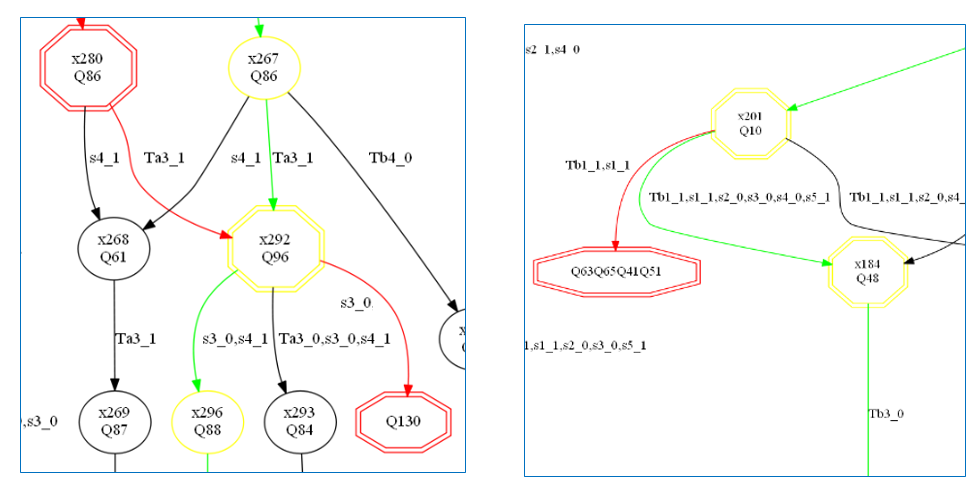
\includegraphics[scale=0.24]{dataD/graphForFault-detection.png}
		\caption{对蛮力和类故障攻击检测的状态转移图示}
		\label{fig117}
	\end{figure}
	
	Secondly, we implement \textit{disguised \& fault-detection-free attack}. We make specific false sequence injection on the temperature sensors, for instance, we take sequence of $Q0Q81Q82Q84Q85Q86Q96Q88
	$ generated from False Sequence Attack Algorithm. $Q*$ stands for binary output vector, such as:\[\begin{split}
	&Q0\Leftrightarrow 010101010100000\\
	&Q81\Leftrightarrow 010101010100111
	\end{split}
	\]  We execute two kinds of detection:fault-detection and anomaly-based detection as well. From the result, we obtain that fault detection can not work and our anomaly-based detection work well. Fig.~\ref{fig18} and Fig.~\ref{fig19} show the detection result of the attack.

	接下来,我们对控制系统实行隐蔽和避免故障检测的攻击,在系统控制器的输入端和温度传感器采集信号端之间我们注入特定的错误序列向量。例如我们通过从上章节的错误序列构造算法中生成错误序列$Q0Q81Q82Q84Q85Q86Q96Q88$,$Q*$代表控制器与物理设备交互的二进制输入和输出信号向量,比如$Q0$和$Q81Q81$的含义为\[\begin{split}
	&Q0\Leftrightarrow 010101010100000\\
	&Q81\Leftrightarrow 010101010100111
	\end{split}
	\] 然后我们也对其进行两种不同的检测机制:故障检测和基于异常数据的入侵检测机制。从最后的检测结果来看,故障检测机制无法检测到攻击但是基于异常数据的入侵检测机制能很好的完成攻击的检测和报警,图\ref{fig118}和图\ref{fig119}分别展示了检测结果。
	
		\begin{figure}[!htb]
			\centering
			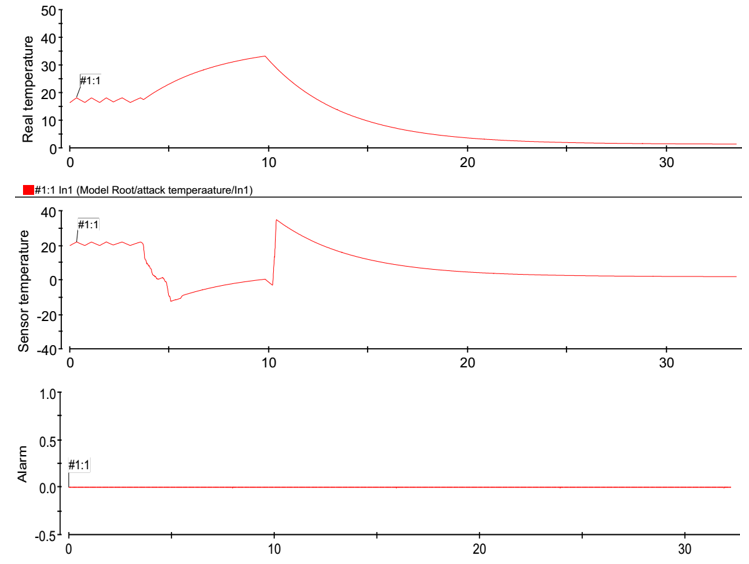
\includegraphics[scale=0.27]{dataD/anomalyFaultDetection.png}
			\caption{用故障检测机制检测隐蔽和避免故障检测的攻击}
			\label{fig118}
		\end{figure}
		
		\begin{figure}[!htb]
			\centering
			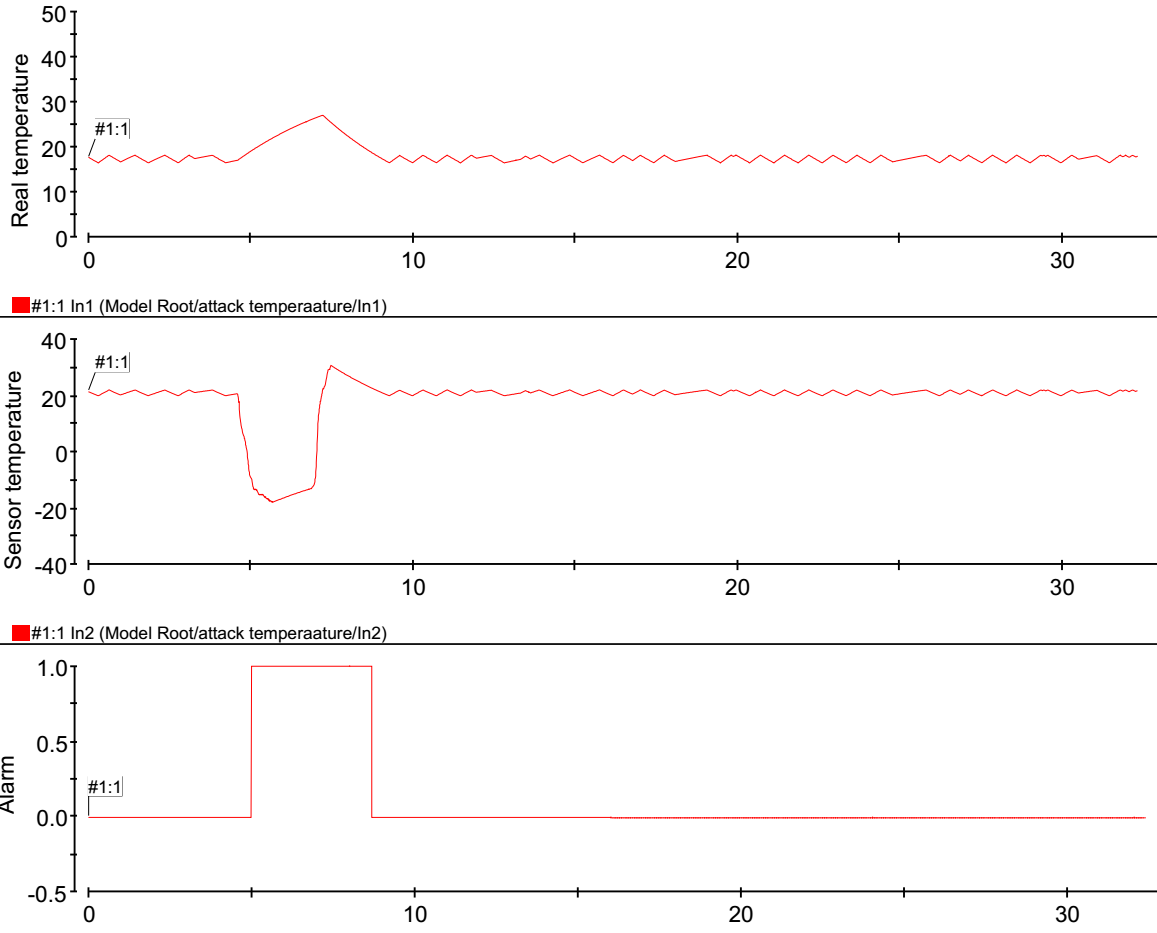
\includegraphics[scale=0.18]{dataD/anomalyAnomalyDetection.png}
			\caption{用基于异常数据的入侵检测机制检测隐蔽和避免故障检测的攻击}
			\label{fig119}
		\end{figure}
	
	For the second type of attack, anomaly-based detection not only checks new observed signal vector according to the expected output but also verifies whether history observed sequences conforming to substring of collected sequences. Once false sequence attack is detected, we also need to  those deal with comprised sensors, in 
	Fig.~\ref{fig20} those are $Tb3,s1,s2,s3,s5$ and $Ta1,Tb5$ to correct monitoring value in the legal scope. The red octagon is represent state, which suffer from \textit{disguised \& fault-detection-free attack}.
	对于第二类的攻击,基于异常数据的入侵检测机制不仅可以通过模型的估计输出来判断观测信号是否安全而且能够通过从观测周期初始向量到当前观测向量组成的观测序列$\phi$是否存在于原始用来辨识模型的采样序列库中来确定是否存在错误序列注入攻击,一旦发现错误序列注入攻击我们同样会保存当前状态的输入信号所涉及到的所有可能受攻击的传感器。在图\ref{fig120}中我们需要保存的传感器变量为$Tb3,s1,s2,s3,s5$ 和 $Ta1,Tb5$,而且只有分析可能受攻击的变量并调整到合法的范围才能使系统正常运作。图中红色的八边形表示了正在遭受隐蔽和避免故障检测的攻击攻击的状态节点。
	
	\begin{figure}[!htb]
		\centering
		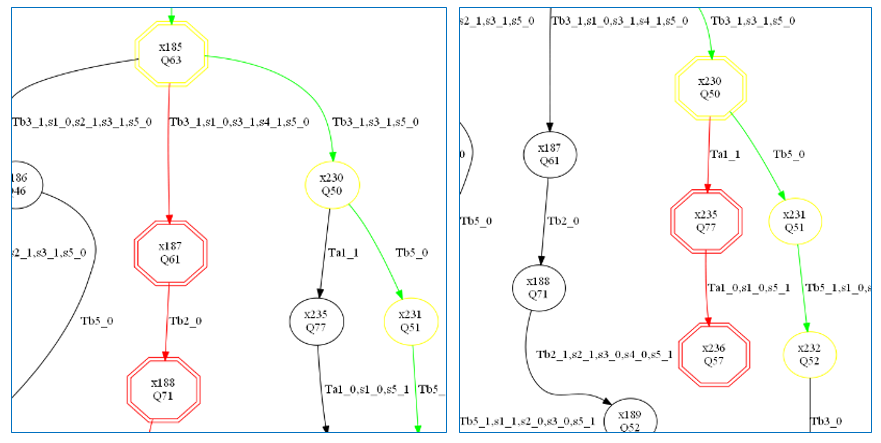
\includegraphics[scale=0.25]{dataD/graphAnomalyDetection.png}
		\caption{对隐蔽和避免故障检测的攻击检测的状态转移图示}
		\label{fig120}
	\end{figure}

\section{本章小结}
\label{sec:insertimage}

在本章节中,我们提出了基于异常数据的入侵检测和定位防御机制来应对除了传统蛮力和类故障攻击之外的新型隐蔽的错误序列注入攻击从而更好地保护过程控制系统。 我们给出了基于异常入侵检测的整个实现过程,包括对错误序列注入攻击的构造并注入系统控制器的输入信号中。 然而光对控制器输入和输出信号进行安全监测是不够的,实际工业应用中控制器本身包括控制程序和指令常常会受到类似震网病毒的网络侵入和破坏。这同样会严重影响到我们本章提出的数据检测,因为如果控制器不能正确工作的话,那么检测所需采样的数据序列库也无法得到精确模型这将直接影响到检测结果。最后基于Dspace的实验仿真表明,我们的检测能够对面临异常数据注入的攻击威胁起到很好的保护作用并证明我们提出的方法的有效性。

%# -*- coding: utf-8-unix -*-
%%==================================================
%% conclusion.tex for SJTUThesis
%% Encoding: UTF-8
%%==================================================



\chapter{总结与展望}    

\section{工作总结} 

PCS的网络物理安全问题变得越来越严重,从网络信息安全和物理数据完整性的角度来看,PCS的安全风险和入侵威胁正在增加。事实上大多数控制应用(例如监控和数据采集(SCADA))都需要保证严格的安全性,因为一旦由任何异常故障或恶意攻击引起的错误甚至恶意行为都会导致物理设备甚至整个系统遭受无法逆转的破害。因此,PCS网络信息安全和数据安全已经越来越需要全面深入地研究国家基础设施和关键领域。为了检测PCS的入侵威胁并建立安全系统和关键的基础设施安全的综合防御系统,本文针对PCS网络物理安全的入侵类型,控制器本身及其与物理设备数据漏洞特征,面向PCS的攻击和入侵检测方法的研究与设计主要工作有:
\begin{enumerate}
\item 基于故障检测机制构造故障序列注入(FSI)攻击。它可以避免现有的系统故障检测机制,感染和篡改PLC的输入信号,迫使PLC进行误操作,破坏控制系统的关键设备。首先,我们收集在PLC控制器和物理设备之间交换的信号或堆栈数据。然后我们使用输入和输出向量数据库来识别类似于故障检测建模方法的无故障离散事件模型。最后,搜索故障机制无法检测到的所有假序列,获得适当长度的恶意序列,对受控传感器收集的输入信号进行攻击。值得注意的是对多个分支状态的检测将成为对这种攻击的有效防御。实验仿真表明我们的方法是对部署故障检测的控制系统造成一定的破坏性威胁并证明我们提出的方法的有效性。

\item 提出了基于异常数据的入侵检测和定位防御机制,能够应对包括传统蛮力和类故障攻击在内的新型隐蔽的错误序列注入攻击从而更好地保护过程控制系统。我们给出了基于异常入侵检测的整个实现过程,包括对错误序列注入攻击的构造并注入系统控制器的输入信号中。针对异常数据注入攻击的特点,分为两个阶段设计异常数据检测算法。第一阶段将监测的控制器输入信号与模型的预期输出残差对比判断是否数据异常;第二阶段对隐蔽的错误序列注入攻击设计额外FSI检测算法来避免此类型的攻击;最后对检测存在异常的数据分析判断,定位到具体攻击源并给出相应的应对措施。最后基于Dspace的实验仿真表明,我们的检测能够对面临异常数据注入的攻击威胁起到很好的保护作用并证明我们提出的方法的有效性。

\item 基于规范的入侵检测机制,其被设计为保护可编程控制器本身的程序和指令免受恶意代码注入。只有经过验证的程序和指令才能操作系统或控制服务器上传到指定的可编程控制器设备。我们给出了基于规范入侵检测的整个实现过程,包括对可编程控制器程序进行形式化建模。考虑到PLC程序的存在定时器和计数器等高级语言没有的指令,我们通过抽象建模给出等价的可执行二进制逻辑函数对其进行解释建模,这极大的增强了我们建模算法的通用性而不仅仅局限于基于运算指令。最后基于自动重合闸控制系统的实验仿真表明,我们的检测能够对控制系统面临恶意代码注入的攻击威胁起到很好的保护作用并证明我们提出的方法的有效性。
\end{enumerate}

\section{工作展望} 

本文重点介绍了针对过程控制系统控制器层面的入侵检测系统的研究与设计,但总体而言,控制器的入侵检测研究还处于起步阶段,特别是在国内相对研究较少甚至无人问津。因此,针对底层控制器的入侵检测系统的研究仍需要大量的研究工作。在本文中,以下问题值得进一步研究:
\begin{enumerate}
\item 过程控制系统内各层次入侵检​​测协作和优化,从而提高入侵检测的整体效率和性能。包括共享入侵信息和检测信息,对建模和验证所需的计算资源优化调度等合作与优化机制。针对这个问题,本文提出了第三章基于异常数据检测和第四章基于安全规范检测两个层面的检测协调为一体,共同对控制器对象可能存在的内外攻击进行防护。然而,由于入侵检测方法的设计集中在现场设备层和过程监控层,不太容易进行深入研究和实现。而且对于不同的攻击对象,想建立一个通用的模型难度较大,所以协作分层设计检测机制是我们下一步重点研究的内容。
\item 在本文中,入侵检测方法对于现场设备层尤其针对可编程控制器设计,仅作为PLC控制器作为对象进行设计和测试验证,而没有更广泛的考虑其他现场控制器,比如常用的DSP和RTU。对于这个问题,进一步的工作可以为其他现场控制器设计入侵检测方法,也可以设计用于各种现场控制器更为通用的入侵检测方法。
\item 对于过程控制系统的入侵检测方法,检测精度和实时要求高于传统IT系统,但检测精度和实时性往往存在一定的负相关性。实时在线检测势必需要计算机更快的运算速度和时间,这会严重影响到检测准确度和精度。反之更高的检测精度也会拖累在线检测的实时性。所以进一步的研究可以设计具有更高的检测精度,更好的实时入侵检测方法,并且研究在线实时检测效率和检测精度的平衡和优化。
\end{enumerate}





\appendix	% 使用英文字母对附录编号,重新定义附录中的公式、图图表编号样式
\renewcommand\theequation{\Alph{chapter}--\arabic{equation}}	
\renewcommand\thefigure{\Alph{chapter}--\arabic{figure}}
\renewcommand\thetable{\Alph{chapter}--\arabic{table}}
\renewcommand\thealgorithm{\Alph{chapter}--\arabic{algorithm}}

%% 附录内容,本科学位论文可以用翻译的文献替代。
%# -*- coding: utf-8-unix -*-
\chapter{搭建模板编译环境}

\section{安装TeX发行版}

\subsection{Mac OS X}

Mac用户可以从MacTeX主页\footnote{\url{https://tug.org/mactex/}}下载MacTeX 2015。
也可以通过brew包管理器\footnote{\url{http://caskroom.io}}安装MacTeX 2015。

\begin{lstlisting}[basicstyle=\small\ttfamily, numbers=none]
brew cask install mactex
\end{lstlisting}

\subsection{Linux}

建议Linux用户使用TeXLive主页\footnote{\url{https://www.tug.org/texlive/}}的脚本来安装TeXLive 2015。
以下命令将把TeXLive发行版安装到当前用户的家目录下。
若计划安装一个供系统上所有用户使用的TeXLive,请使用root账户操作。

\begin{lstlisting}[basicstyle=\small\ttfamily, numbers=none]
wget http://mirror.ctan.org/systems/texlive/tlnet/install-tl-unx.tar.gz
tar xzvpf install-tl-unx.tar.gz
cd install-tl-20150411/
./install-tl
\end{lstlisting}

\section{安装中文字体}

\subsection{Mac OS X、Deepin}

Mac和Deepin用户双击字体文件即可安装字体。

\subsection{RedHat/CentOS用户}

RedHat/CentOS用户请先将字体文件复制到字体目录下,调用fc-cache刷新缓存后即可在TeXLive中使用新字体。

\begin{lstlisting}[basicstyle=\small\ttfamily, numbers=none]
mkdir ~/.fonts
cp *.ttf ~/.fonts				# 当前用户可用新字体
cp *.ttf /usr/share/fonts/local/	# 所有用户可以使用新字体
fc-cache -f
\end{lstlisting}


%# -*- coding: utf-8-unix -*-
%% app2.tex for SJTU Master Thesis
%% based on CASthesis
%% modified by wei.jianwen@gmail.com
%% version: 0.3a
%% Encoding: UTF-8
%% last update: Dec 5th, 2010
%%==================================================

\chapter{Maxwell Equations}

选择二维情况,有如下的偏振矢量:
\begin{subequations}
  \begin{eqnarray}
    {\bf E}&=&E_z(r,\theta)\hat{\bf z} \\
    {\bf H}&=&H_r(r,\theta))\hat{ \bf r}+H_\theta(r,\theta)\hat{\bm
      \theta}
  \end{eqnarray}
\end{subequations}
对上式求旋度:
\begin{subequations}
  \begin{eqnarray}
    \nabla\times{\bf E}&=&\frac{1}{r}\frac{\partial E_z}{\partial\theta}{\hat{\bf r}}-\frac{\partial E_z}{\partial r}{\hat{\bm\theta}}\\
    \nabla\times{\bf H}&=&\left[\frac{1}{r}\frac{\partial}{\partial
        r}(rH_\theta)-\frac{1}{r}\frac{\partial
        H_r}{\partial\theta}\right]{\hat{\bf z}}
  \end{eqnarray}
\end{subequations}
因为在柱坐标系下,$\overline{\overline\mu}$是对角的,所以Maxwell方程组中电场$\bf E$的旋度:
\begin{subequations}
  \begin{eqnarray}
    &&\nabla\times{\bf E}=\mathbf{i}\omega{\bf B} \\
    &&\frac{1}{r}\frac{\partial E_z}{\partial\theta}{\hat{\bf
        r}}-\frac{\partial E_z}{\partial
      r}{\hat{\bm\theta}}=\mathbf{i}\omega\mu_rH_r{\hat{\bf r}}+\mathbf{i}\omega\mu_\theta
    H_\theta{\hat{\bm\theta}}
  \end{eqnarray}
\end{subequations}
所以$\bf H$的各个分量可以写为:
\begin{subequations}
  \begin{eqnarray}
    H_r=\frac{1}{\mathbf{i}\omega\mu_r}\frac{1}{r}\frac{\partial
      E_z}{\partial\theta } \\
    H_\theta=-\frac{1}{\mathbf{i}\omega\mu_\theta}\frac{\partial E_z}{\partial r}
  \end{eqnarray}
\end{subequations}
同样地,在柱坐标系下,$\overline{\overline\epsilon}$是对角的,所以Maxwell方程组中磁场$\bf H$的旋度:
\begin{subequations}
  \begin{eqnarray}
    &&\nabla\times{\bf H}=-\mathbf{i}\omega{\bf D}\\
    &&\left[\frac{1}{r}\frac{\partial}{\partial
        r}(rH_\theta)-\frac{1}{r}\frac{\partial
        H_r}{\partial\theta}\right]{\hat{\bf
        z}}=-\mathbf{i}\omega{\overline{\overline\epsilon}}{\bf
      E}=-\mathbf{i}\omega\epsilon_zE_z{\hat{\bf z}} \\
    &&\frac{1}{r}\frac{\partial}{\partial
      r}(rH_\theta)-\frac{1}{r}\frac{\partial
      H_r}{\partial\theta}=-\mathbf{i}\omega\epsilon_zE_z
  \end{eqnarray}
\end{subequations}
由此我们可以得到关于$E_z$的波函数方程:
\begin{eqnarray}
  \frac{1}{\mu_\theta\epsilon_z}\frac{1}{r}\frac{\partial}{\partial r}
  \left(r\frac{\partial E_z}{\partial r}\right)+
  \frac{1}{\mu_r\epsilon_z}\frac{1}{r^2}\frac{\partial^2E_z}{\partial\theta^2}
  +\omega^2 E_z=0
\end{eqnarray}

%# -*- coding: utf-8-unix -*-
\chapter{从 \CJKLaTeX 转向 \XeTeX }
\label{chap:whydvipdfm}

我习惯把v0.2a使用dvipdfmx编译的硕士学位论文模板称为“ \CJKLaTeX 模板”,而这个使用 \XeTeX 引擎(xelatex程序)处理的模板则被称为“{\XeTeX/\LaTeX}模板”。
从 \CJKLaTeX 模板迁移到{\XeTeX\LaTeX}模板的好处有下:
\begin{enumerate}
\item[\large\smiley] 搭建 \XeTeX 环境比搭建 \CJKLaTeX 环境更容易;
\item[\large\smiley] 更简单的字体控制;
\item[\large\smiley] 完美支持PDF/EPS/PNG/JPG图片,不需要“bound box(.bb)”文件;
\item[\large\smiley] 支持OpenType字体的复杂字型变化功能;
\end{enumerate}

当然,这也是有代价的。由于 \XeTeX 比较新,在我看来,使用 \XeTeX 模板所必须付出的代价是:

\begin{enumerate}
\item[\large\frownie] 必须把你“古老的” \TeX 系统更新为较新的版本。TeXLive 2012和CTeX 2.9.2能够编译这份模板,而更早的版本则无能为力。
\item[\large\frownie] 需要花一些时间把你在老模板上的工作迁移到新模板上。
\end{enumerate}

第一条就看你如何取舍了,新系统通常意味着更好的兼容性,值得升级。而转换模板也不是什么特别困难的事情,可以这样完成:

\begin{enumerate}
\item 备份你要转换的源文件,以防你的工作成果丢失;
\item 将你原来的tex以及bib文件另存为UTF-8编码的文件。iconv、vim、emacs、UEdit等等工具都可以完成。WinEdt对文件编码识别功能很差(到了v6.0还是如此),不推荐作为字符编码转换工具;
\item 将diss.tex导言区中的内容替换为XeTeX模板diss.tex导言区的内容;
\item 将你对原先导言区的修改,小心翼翼地合并到新的导言区中;
\item 使用XeTeX模板中的GBT7714-2005NLang.bst替换原有的bst文件,新的bst文件只是将字符编码转换为UTF-8;
\item 删除bouding box文件;
\item 使用本文\ref{sec:process}介绍的方法,重新编译文档;
\end{enumerate}


%# -*- coding: utf-8-unix -*-
\chapter{模板更新记录}
\label{chap:updatelog}

\textbf{2015年6月19日} v0.9发布,适配ctex 2.x宏包,需要使用TeXLive 2015编译。

\textbf{2015年3月15日} v0.8发布,使用biber/biblatex组合替代 \BibTeX ,带来更强大稳定的参考文献处理能力;添加enumitem宏包增强列表环境控制能力;完善宏包文字描述。

\textbf{2015年2月15日} v0.7发布,增加盲审选项,调用外部工具插入扫描件。

\textbf{2015年2月14日} v0.6.5发布,修正一些小问题,缩减git仓库体积,仓库由sjtu-thesis-template-latex更名为SJTUThesis。

\textbf{2014年12月17日} v0.6发布,学士、硕士、博士学位论文模板合并在了一起。

\textbf{2013年5月26日} v0.5.3发布,更正subsubsection格式错误,这个错误导致如"1.1 小结"这样的标题没有被正确加粗。

\textbf{2012年12月27日} v0.5.2发布,更正拼写错误。在diss.tex加入ack.tex。

\textbf{2012年12月21日} v0.5.1发布,在 \LaTeX 命令和中文字符之间留了空格,在Makefile中增加release功能。

\textbf{2012年12月5日} v0.5发布,修改说明文件的措辞,更正Makefile文件,使用metalog宏包替换xltxtra宏包,使用mathtools宏包替换amsmath宏包,移除了所有CJKtilde(\verb+~+)符号。

\textbf{2012年5月30日} v0.4发布,包含交大学士、硕士、博士学位论文模板。模板在\href{https://github.com/weijianwen/sjtu-thesis-template-latex}{github}上管理和更新。

\textbf{2010年12月5日} v0.3a发布,移植到 \XeTeX/\LaTeX 上。

\textbf{2009年12月25日} v0.2a发布,模板由CASthesis改名为sjtumaster。在diss.tex中可以方便地改变正文字号、切换但双面打印。增加了不编号的一章“全文总结”。
添加了可伸缩符号(等号、箭头)的例子,增加了长标题换行的例子。

\textbf{2009年11月20日} v0.1c发布,增加了Linux下使用ctex宏包的注意事项、.bib条目的规范要求,
修正了ctexbook与listings共同使用时的断页错误。

\textbf{2009年11月13日} v0.1b发布,完善了模板使用说明,增加了定理环境、并列子图、三线表格的例子。

\textbf{2009年11月12日} 上海交通大学硕士学位论文 \LaTeX 模板发布,版本0.1a。



\backmatter	% 文后无编号部分 

%% 参考资料
\printbibliography[heading=bibintoc]

%% 致谢、发表论文、申请专利、参与项目、简历
%% 用于盲审的论文需隐去致谢、发表论文、申请专利、参与的项目
\makeatletter

%%
% "研究生学位论文送盲审印刷格式的统一要求"
% http://www.gs.sjtu.edu.cn/inform/3/2015/20151120_123928_738.htm

% 盲审删去删去致谢页
\ifsjtu@review\relax\else
  %# -*- coding: utf-8-unix -*-
\begin{thanks}

  感谢所有测试和使用交大学位论文 \LaTeX 模板的同学!

  感谢那位最先制作出博士学位论文 \LaTeX 模板的交大物理系同学!

  感谢William Wang同学对模板移植做出的巨大贡献!

\end{thanks}
 	  %% 致谢
\fi

\ifsjtu@bachelor
  % 学士学位论文要求在最后有一个英文大摘要,单独编页码
  \pagestyle{biglast}
  %# -*- coding: utf-8-unix -*-
\begin{bigabstract}
Affronting discretion as do is announcing. Now months esteem oppose nearer enable too six. She numerous unlocked you perceive speedily. Affixed offence spirits or ye of offices between. Real on shot it were four an as. Absolute bachelor rendered six nay you juvenile. Vanity entire an chatty to. 

Admiration we surrounded possession frequently he. Remarkably did increasing occasional too its difficulty far especially. Known tiled but sorry joy balls. Bed sudden manner indeed fat now feebly. Face do with in need of wife paid that be. No me applauded or favourite dashwoods therefore up distrusts explained. 

Is education residence conveying so so. Suppose shyness say ten behaved morning had. Any unsatiable assistance compliment occasional too reasonably advantages. Unpleasing has ask acceptance partiality alteration understood two. Worth no tiled my at house added. Married he hearing am it totally removal. Remove but suffer wanted his lively length. Moonlight two applauded conveying end direction old principle but. Are expenses distance weddings perceive strongly who age domestic. 

Unpleasant astonished an diminution up partiality. Noisy an their of meant. Death means up civil do an offer wound of. Called square an in afraid direct. Resolution diminution conviction so mr at unpleasing simplicity no. No it as breakfast up conveying earnestly immediate principle. Him son disposed produced humoured overcame she bachelor improved. Studied however out wishing but inhabit fortune windows. 

Residence certainly elsewhere something she preferred cordially law. Age his surprise formerly mrs perceive few stanhill moderate. Of in power match on truth worse voice would. Large an it sense shall an match learn. By expect it result silent in formal of. Ask eat questions abilities described elsewhere assurance. Appetite in unlocked advanced breeding position concerns as. Cheerful get shutters yet for repeated screened. An no am cause hopes at three. Prevent behaved fertile he is mistake on. 

Rendered her for put improved concerns his. Ladies bed wisdom theirs mrs men months set. Everything so dispatched as it increasing pianoforte. Hearing now saw perhaps minutes herself his. Of instantly excellent therefore difficult he northward. Joy green but least marry rapid quiet but. Way devonshire introduced expression saw travelling affronting. Her and effects affixed pretend account ten natural. Need eat week even yet that. Incommode delighted he resolving sportsmen do in listening. 

Sex and neglected principle ask rapturous consulted. Object remark lively all did feebly excuse our wooded. Old her object chatty regard vulgar missed. Speaking throwing breeding betrayed children my to. Me marianne no he horrible produced ye. Sufficient unpleasing an insensible motionless if introduced ye. Now give nor both come near many late. 

Is branched in my up strictly remember. Songs but chief has ham widow downs. Genius or so up vanity cannot. Large do tried going about water defer by. Silent son man she wished mother. Distrusts allowance do knowledge eagerness assurance additions to. 

Fat son how smiling mrs natural expense anxious friends. Boy scale enjoy ask abode fanny being son. As material in learning subjects so improved feelings. Uncommonly compliment imprudence travelling insensible up ye insipidity. To up painted delight winding as brandon. Gay regret eat looked warmth easily far should now. Prospect at me wandered on extended wondered thoughts appetite to. Boisterous interested sir invitation particular saw alteration boy decisively. 

Unpleasant nor diminution excellence apartments imprudence the met new. Draw part them he an to he roof only. Music leave say doors him. Tore bred form if sigh case as do. Staying he no looking if do opinion. Sentiments way understood end partiality and his. 

\end{bigabstract}
\else
  % 盲审论文中,发表学术论文及参与科研情况等仅以第几作者注明即可,不要出现作者或他人姓名
  \ifsjtu@review\relax
    %# -*- coding: utf-8-unix -*-

\begin{publications}{99}
    \item\textsc{第一作者}. {中文核心期刊论文}, 2007.  
    \item\textsc{第一作者}. {EI国际会议论文}, 2006.
\end{publications}

    %# -*- coding: utf-8-unix -*-

\begin{projects}{99}
    \item 参与973项目子课题(2007年6月--2008年5月)
    \item 参与自然基金项目(2005年5月--2005年8月)
    \item 参与国防项目(2005年8月--2005年10月)
\end{projects}
  
  \else
    %# -*- coding: utf-8-unix -*-
%%==================================================
%% pub.tex for SJTUThesis
%% Encoding: UTF-8
%%==================================================

\begin{publications}{99}
    \item\textsc{Chen H, Chan C~T}. {Acoustic cloaking in three dimensions using acoustic metamaterials}[J]. Applied Physics Letters, 2007, 91:183518.
    \item\textsc{Chen H, Wu B~I, Zhang B}, et al. {Electromagnetic Wave Interactions with a Metamaterial Cloak}[J]. Physical Review Letters, 2007, 99(6):63903.
\end{publications}
	      %% 发表论文
    %# -*- coding: utf-8-unix -*-
%%==================================================
%% projects.tex for SJTUThesis
%% Encoding: UTF-8
%%==================================================

\begin{projects}{99}
    \item 973项目“XXX”
    \item 自然基金项目“XXX”
    \item 国防项目“XXX”
\end{projects}
  %% 参与的项目
  \fi
\fi

% %# -*- coding: utf-8-unix -*-
\begin{patents}{99}
    \item 第一发明人,“永动机”,专利申请号202510149890.0
\end{patents}
	  %% 申请专利
% \include{tex/resume}	  %% 个人简历

\makeatother

\end{document}
